\documentclass[a4paper,12pt,titlepage]{book}

\usepackage{fancyhdr}
\usepackage[swapnames]{frontespizio}
\usepackage[italian]{babel}
\usepackage[T1]{fontenc}
% \usepackage[latin1]{inputenc}
\usepackage[utf8]{inputenc}
\usepackage{csquotes}
\usepackage[bookmarks]{hyperref}
\usepackage{amsmath}
\usepackage{verbatim} % citazioni
\usepackage{booktabs}
\usepackage{url}
\usepackage{listings} % code
\usepackage{booktabs} % tables
\usepackage[style=numeric, backend=biber]{biblatex}
\usepackage{wrapfig} % immagini allineate con testo
\graphicspath{ {img/} {imgtesi/} }
\newcommand{\dd}[1]{\mathrm{d}#1} % numerare formule

\addbibresource{bibliografia.bib} 

%%%% ABSTRACT DEFINITION
\newenvironment{abstract} %
{\cleardoublepage %
\thispagestyle {empty} %
\null \vfill \begin{center} %
\bfseries \abstractname \end {center}} %
{\vfill \null }


\begin{document}

\begin{frontespizio}
\Logo{./img/logo_uniba}
\Universita{Bari}
\Dipartimento{Informatica}
\Corso[Laurea Triennale]{Informatica}
\Annoaccademico{2013 -- 2014}
\Titolo{Piattaforma cloud per l'analisi di big data

provenienti da social network}
\Sottotitolo{Tecnologie per l'individuazione di contenuti a sfondo discriminatorio}
\Candidato[587176]{Gianvito Taneburgo}
\Relatore{Prof. Pasquale Lops}
\Relatore{Dott. Pierpaolo Basile}
\end{frontespizio} 

\renewcommand{\baselinestretch}{0.95}\normalsize
\tableofcontents
\renewcommand{\baselinestretch}{1.0}\normalsize

\part{Prefazione}

\chapter*{Introduzione}
\addcontentsline{toc}{chapter}{Introduzione} 

% \cite{google:filesystem} 

% \includegraphics{prova}

% \begin{figure}[h]
% \centering
% \includegraphics{prova.jpg}
% \caption{Example of a parametric plot}
% \end{figure}

% \begin{wrapfigure}{r}{0.25\textwidth} %this figure will be at the right
%     \centering
%     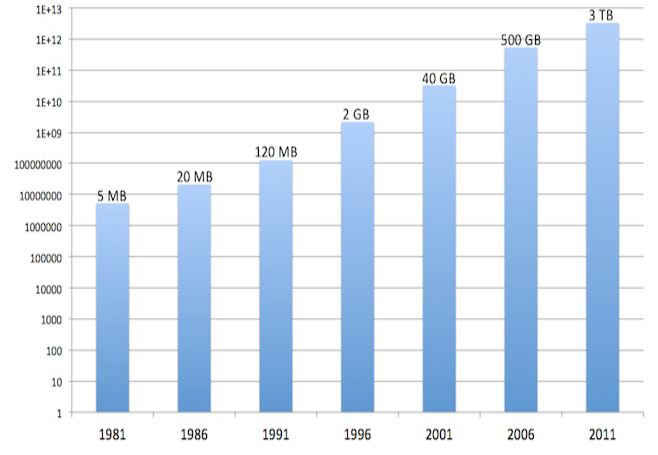
\includegraphics[width=0.25\textwidth]{harddisk}
%     \caption{Example of a parametric plot}
% \end{wrapfigure}

Il progresso tecnologico degli ultimi anni ha rivoluzionato il modo con cui gli esseri umani conoscono, lavorano, si relazionano con gli altri e, più in generale, interagiscono 
in un contesto sociale. Il fattore decisivo per questo cambiamento è stato Internet, la più grande rete di computer del mondo, accessibile dal 40\% circa della popolazione 
mondiale \cite{URL:internetstats}.

Nato nel 1991 per opera di Tim Berners-Lee, il World Wide Web si è evoluto molto velocemente fino a diventare la più ricca sorgente di informazioni della storia dell’uomo, 
accessibile consultando liberamente miliardi di pagine web. Lo sviluppo di complesse tecnologie e di nuove tecniche di programmazione ha radicalmente modificato la struttura 
di queste pagine, che hanno perso la loro natura statica per acquisirne una notevolmente più dinamica. Gli utenti del Web hanno così potuto cominciare ad interagire con le 
pagine visualizzate ed a contribuire in prima persona alla pubblicazione di nuovi contenuti. In questa maniera si sono sviluppate nuove tipologie di siti, come 
forum, blog, chat, \textit{wiki} e, solo in tempi più recenti, \textbf{\textit{social network}}. La trasformazione è stata così profonda da indurre all’utilizzo dell’espressione \textit{Web 2.0}
per descrivere la nuova forma del più celebre servizio di Internet.

Ciascun individuo ha acquisito primaria importanza nell’era dell’informazione (non a caso la rivista TIME ha scelto \textit{You} come persona dell'anno 
nel 2006 \cite{URL:TIME1}\cite{URL:TIME2}), 
trasformandosi da semplice fruitore di contenuti in sorgente copiosa di nuovi dati. Diversi fattori hanno, inoltre, contribuito alla crescita della mole di informazioni condivise in rete: lo sviluppo degli 
smartphone e delle reti di comunicazione digitali per telefonia mobile, l’aumento della velocità media di connessione ad Internet, la presenza di sensori in molti dispositivi di uso quotidiano, ecc.
Il volume di dati prodotti è così aumentato a dismisura col passare degli anni, avviando quella che viene definita da alcuni come \textit{era dei \textbf{big data}}.

Le informazioni generate si sono concentrate nei \textit{data center} dei colossi dell’\textit{Information Technology} (IT) proprietari dei siti web più visitati, che 
le hanno utilizzate per creare nuove ed abbondanti fonti di guadagno, accrescendo ricchezza, fama e potere in modo proporzionale 
al volume dei dati posseduti. Non stupisce, pertanto, notare come molti degli imprenditori più ricchi del pianeta dirigano proprio queste aziende \cite{URL:top30ent}, nè stupisce osservare 
nelle prime posizioni della classifica dei siti web più popolari al mondo \cite{URL:alexatop} i \textit{social network}, servizi che aggregano milioni di utenti al fine di costituire una rete sociale virtuale.
Tra questi spiccano su tutti Facebook e Twitter che sono stati protagonisti di una espansione imponente, superando la complessa fase di \textit{start up} per merito soprattutto
della loro semplicità d'uso e dell'innovazione portata nel panorama dei siti web preesistenti.
Questa improvvisa ed inaspettata crescita ha però presentato diverse sfide alle aziende proprietarie dei rispettivi siti: tutela della privacy degli utenti, recupero delle spese
di gestione, design di interfacce facilmente usabili da individui profondamente diversi tra loro, ecc. La prova più complessa affrontata è stata certamente 
sviluppare \textbf{infrastrutture scalabili e performanti}, adatte a gestire enormi bacini di utenza e di dati. Quest’ultima è stata superata dagli \textit{entrepreneur} 
per merito di avanzate tecnologie progettate appositamente per \textbf{memorizzare} ed \textbf{elaborare} \textit{big data}.

Tali tecnologie sono state oggetto di approfondimento per questo caso di studio e, successivamente, sono state impiegate per lo sviluppo di una \textbf{piattaforma \textit{cloud}} per l’analisi di grandi moli 
di dati provenienti da \textit{social network}. Tale piattaforma è stata progettata per essere di supporto alla Mappa dell’Intolleranza, uno strumento promosso da Vox, Osservatorio 
Italiano sui Diritti, per monitorare le zone dove omofobia, razzismo, odio verso i disabili, misoginia ed antisemitismo sono maggiormente diffusi
nel nostro Paese. La Mappa dell’Intolleranza, infatti, evidenzia i luoghi affetti da questi gravi problemi di discriminazione mediante l'uso di una mappa di calore 
dell’Italia, ottenuta analizzando i messaggi geolocalizzati inviati dal nostro Paese su Twitter. Quest'ultimo, più di tutti gli altri \textit{social network}, si presta facilmente a veicolare messaggi
d'odio, che richiedono, inoltre, accorgimenti particolari in fase di analisi per la loro peculiare natura (\textit{hasthag}, menzioni, \textit{emoticon}, link, ecc.). 
Una volta completato, lo strumento potrebbe essere usato per informare le amministrazioni locali delle città più a rischio, al fine di agire con interventi mirati sul territorio e
prevenire l'insorgere di episodi spiacevoli.

Un sistema che mira ad analizzare velocemente, se non in \textit{real-time}, i \textit{tweet} inviati in Italia necessita di una infrastruttura scalabile, in grado di gestire una quantità enorme 
di dati. A questa esigenza prova a dare una soluzione la piattaforma sviluppata per il caso di studio, adoperando tecnologie specifiche per memorizzare e 
processare \textit{big data} in tempi ristretti. Con l'obiettivo di massimizzare l'efficacia degli strumenti utilizzati, è stata progettata una architettura che si avvale di servizi \textit{cloud} per portare a termine i compiti più esosi di risorse.
Dopo diverse analisi, Google è stato selezionato 
come il \textit{cloud provider} ideale per il caso di studio. La piattaforma sviluppata, pertanto, impiega nel suo \textit{core} alcuni prodotti della Google Cloud Platform, un portfolio di 
soluzioni \textit{cloud} utilizzanti le stesse infrastrutture del motore di ricerca e degli altri prodotti di Google, come Gmail e YouTube.

Oltre ad essere stato adoperato per la raccolta di dati dal \textit{social network}, il sistema è stato anche impiegato per migliorare il procedimento 
di individuazione dei \textit{tweet} discriminatori tra quelli nel flusso di messaggi, conducendo indagini di natura statistica su quelli raccolti. L’obiettivo di questa analisi è stato quello di individuare
i termini tipicamenti utilizzati nei \textit{tweet} connotati da determinate forme di intolleranza, ma generalmente poco riccorenti in generici testi in lingua italiana. Coi risultati
del lavoro si potrebbe rendere più mirata la raccolta di informazioni da mostrare sulla Mappa dell’Intolleranza, che risulterebbe quindi più accurata ed informativa.

Per la parte sperimentale del caso di studio sono stati progettati ed eseguiti due esperimenti. Il primo mira a confrontare le prestazioni ottenute da una macchina locale con quelle 
fatte registrare da \textit{cluster} di computer in esecuzione sull'infrastruttura di Google, provando configurazioni variabili sia per numero di nodi interconnessi, sia per tipologia di macchine avviate.
Analizzando i tempi necessari per completare lo stesso \textit{task} di indicizzazione è stato possibile valutare quando le tecnologie per il calcolo distribuito si rivelano una soluzione consigliabile e quando si 
dimostrano inefficienti. Il secondo esperimento, invece, si pone come obiettivo quello di evidenziare i termini più peculiari nei messaggi con contenuto potenzialmente intollerante verso il prossimo.
Per eseguirlo è stata calcolata la divergenza di Kullback-Leibler tra i \textit{tweet} collezionati ed il corpus itWaC, una grande raccolta di testi in lingua italiana. I risultati delle analisi hanno 
permesso di comprendere quali contenuti ricorrono con più frequenza nei messaggi ed hanno suggerito dei metodi per migliorare la raccolta futura di nuovi dati.

\chapter*{Sommario}
\addcontentsline{toc}{chapter}{Sommario}

Di seguito viene illustrata per sommi capi la struttura del lavoro.

Per via dell'importanza che rivestono in questo caso di studio, il capitolo \ref{chap:bigdata} è dedicato esclusivamente alla descrizione dei \textit{big data}. Sono analizzati i fattori 
che hanno permesso il loro sviluppo, le sorgenti contemporanee di nuove informazioni, con particolare riguardo per i \textit{social network}, e le possibilità di profitto originabili dal loro impiego. Vengono, infine, spiegate le due criticità principali che emergono quando si gestiscono \textit{big data}: l’elaborazione 
e la memorizzazione.

Per risolvere il primo problema, nel capitolo \ref{chap:hadoop} viene illustrato il funzionamento di Hadoop, un \textit{framework} per il calcolo distribuito attraverso \textit{cluster} di computer.
Nel corso del capitolo vengono approfonditi il \textit{file system} distribuito condiviso dai nodi, il modello di programmazione MapReduce da seguire nella 
scrittura di programmi per il \textit{framework}, i principi di funzionamento alla base della tecnologia e le possibilità a disposizione degli sviluppatori per migliorare le prestazioni dei \textit{cluster}.

Il capitolo \ref{chap:nosql} è destinato alla descrizione dei database NoSQL, una nuova tipologia di database, progettata per memorizzare grandi moli di informazioni.
Nel capitolo vengono illustrate le origini di questi database e, successivamente, viene effettuato un confronto con 
i database relazioni e quelli NewSQL, al fine di evidenziare i punti di forza e di debolezza di ogni tecnologia. Conclude il capitolo la descrizione della tassonomia 
dei database NoSQL.

Il capitolo \ref{chap:cloud} descrive le piattaforme di \textit{cloud computing}, le caratteristiche che generalmente presentano ed i modelli di servizi che offrono ad aziende e privati.
Particolare attenzione viene dedicata alla Google Cloud Platform, la piattaforma \textit{cloud} utilizzata nel caso di studio, 
di cui sono descritti nel dettaglio i due \textit{web service} utilizzati: Compute Engine e Cloud Storage.

La piattaforma \textit{cloud} per l'analisi di \textit{big data} sviluppata per il caso di studio utilizzando le tecnologie finora presentate viene descritta nel capitolo \ref{chap:platform}.
I paragrafi che lo compongono illustrano il contesto del progetto, le finalità del lavoro, l'architettura del sistema ed il funzionamento dei suoi componenti.

Il capitolo \ref{chap:esp} riporta, per entrambi gli esperimenti svolti, una descrizione dei \textit{dataset} di input, il protocollo sperimentale seguito, i risultati ottenuti ed 
una loro discussione.

Completano il lavoro delle sezioni contenenti le conclusioni sul lavoro svolto, i possibili sviluppi futuri del caso di studio ed alcuni sentiti ringraziamenti.

\part{Caso di studio}

\chapter{Big data}
\label{chap:bigdata}

\section{Definizioni}
\label{par:defbigdata}

Con l'espressione \textit{big data} generalmente ci si riferisce ad una grande quantità di dati digitali di varia natura. Tali dati possono essere originati nei 
modi più diversi: transazioni bancarie, cronologie di acquisti su siti di \textit{e-commerce}, registrazioni di fenomeni atmosferici, sms, email, ecc.

Nel condurre uno studio su questi dati risulta inevitabile fare riferimento alle unità di misura dell’informazione digitale. La tabella \ref{table:units}, fedelmente alle indicazioni 
del Sistema internazionale di unità di misura (SI) \cite{bipm}, riporta i multipli del byte che 
saranno incontrati in questo e nei successivi capitoli. La sua consultazione è utile per avere una percezione della dimensione di certe sorgenti informative ed è 
raccomandata ad ogni nuova occorrenza di ordini di grandezza con cui non si ha familiarità.

\begin{table}[ht]
\centering
\begin{tabular}{@{}|l|l|l|@{}}
\toprule
Unità di misura & Simbolo & Valore (byte) \\ \midrule
kilobyte        & kB      & 10\textsuperscript{3}           \\
megabyte        & MB      & 10\textsuperscript{6}           \\
gigabyte        & GB      & 10\textsuperscript{9}           \\
terabyte        & TB      & 10\textsuperscript{12}          \\
petabyte        & PB      & 10\textsuperscript{15}          \\
exabyte         & EB      & 10\textsuperscript{18}          \\
zettabyte       & ZB      & 10\textsuperscript{21}          \\
yottabyte       & YB      & 10\textsuperscript{24}          \\ \bottomrule
\end{tabular}
\caption{ordini di grandezza dei dati.}
\label{table:units}
\end{table}

Definire i \textit{big data} costituisce necessariamente il punto di partenza per l’analisi.

Il modo più semplice per formulare una definizione di \textit{big data} è quello di fissare una soglia oltre la quale un insieme di \textit{data} possa ragionevolmente essere considerato \textit{big}. 
Si potrebbe, ad esempio, affermare che un qualunque insieme di informazioni avente dimensione superiore a 100 PB possa essere etichettato come \textit{big data}. 
Questo approccio quantitativo, sebbene sembri universalmente valido, nasconde diverse insidie. Il primo problema che insorge è quello di riuscire a quantificare 
ragionevolmente questa soglia. Il concetto di \textit{big}, infatti, è assolutamente relativo, poiché fortemente vincolato alle capacità di chi si trova a trattare la mole di dati. 
Un file di \textit{log} contenente 35 milioni di operazioni, infatti, potrebbe risultare difficilmente processabile da un commerciante locale, che probabilmente non venderà tanti oggetti 
in tutto l’arco della sua attività, ed assolutamente ordinario per Amazon, che è ha venduto oltre 37 milioni di prodotti in un solo giorno \cite{URL:cybermon}.
Ma vi è anche un altro problema che deriva da questo approccio: una definizione di \textit{big data} ben 
formulata non dovrebbe essere soggetta ad obsolescenza. Fissando una precisa quantità, invece, si corre il rischio, un domani più o meno prossimo, di avere una definizione
non più valida. Si supponga, infatti, di aver trovato una soglia che oggi risulti adatta ad identificare i \textit{big data}; non serve troppa lungimiranza per comprendere che, 
qualunque essa sia, col passare del tempo essa risulterà inevitabilmente inadatta. La capacità di memorizzazione dei dispositivi, infatti, crescerà continuamente, trasformando 
quelli che avevamo definito come \textit{big data} in dei \textit{not-so-big data}.

Risulta chiaro, da quanto detto, che la definizione di \textit{big data} deve essere inerentemente relativa, per rimanere appropriata, nel corso del tempo, agli strumenti che saranno 
prodotti dal progresso tecnologico. Questa idea è generalmente condivisa da tutti coloro i quali studiano e trattano \textit{big data}.

Tra le tante definizioni di \textit{big data} che è possibile leggere in letteratura, una afferma che si hanno \textit{big data} quando i dati non possono più essere contenuti 
su una singola macchina \cite{hbase:def1}. Tale definizione potrebbe risultare accettabile, poiché è relativa alla capacità di memorizzazione di una macchina, che, 
verosimilmente, aumenterà nel corso degli anni. In tal 
modo, quelli che oggi sono considerati \textit{big data} in futuro non lo saranno più, in favore di \textit{dataset} aventi dimensione maggiore. Una definizione migliore, tuttavia, è la seguente \cite{hbase:def1}:

\begin{lstlisting}[breaklines]
Big Data means the data is large enough that you have to think about it in order to gain insights from it.
\end{lstlisting}

Questa definizione si sofferma non su un aspetto quantitativo, che, come è stato illustrato, può comportare diversi problemi, ma su un aspetto qualitativo, ben più interessante. 
I \textit{big data} vengono definiti tali non più in virtù dello spazio fisico che occupano, ma in relazione alle modalità di gestione che essi richiedono. Si può parlare di \textit{big data} quando 
le informazioni a disposizione sono così tante da richiedere un accurato ragionamento su come utilizzarle per estrarne qualche forma di conoscenza.

Anche l’IBM sottolinea come l’espressione \textit{big data} alluda ad una realtà quotidiana che non lancia una sfida riducibile esclusivamente alla memorizzazione \cite{ibm:def1}:

\begin{lstlisting}[breaklines]
The term "Big Data" is a bit of a misnomer since it implies that preexisting data is somehow  small (it isn't) or that the only challenge is its sheer size (size is one of them, but there are often more).
\end{lstlisting}

Vi è generale consenso sul fatto che i \textit{big data} richiedano un modo sostanzialmente diverso di pensare alle modalità di utilizzo delle informazioni a disposizione, soprattutto se 
l’obiettivo è di trarne profitti.

Gli strumenti adatti all’elaborazione di dati di modeste dimensioni si rivelano del tutto incapaci di trattare \textit{big data}. Apposite tecnologie sono state sviluppate per consentire 
di effettuare su enormi moli di dati le stesse operazioni che solitamente vengono eseguite su campioni più piccoli (acquisizione, memorizzazione, condivisione, analisi e visualizzazione).
Alcuni degli strumenti che permettono di elaborare \textit{big data} saranno analizzati e presentati in questo lavoro.


\section{Fattori di sviluppo}

La disponibilità di una enorme mole di dati che caratterizza i nostri giorni ha origine in una serie di fattori che, sinergicamente, hanno reso possibile la produzione di informazioni 
a ritmi elevatissimi.

Nessuno riuscirebbe, da solo, a generare \textit{big data} in tempi modesti: essi sono il risultato di piccoli contributi di individui sparsi nel mondo. Risulta evidente, pertanto, che il fattore 
principale che ha avviato l’era dei \textit{big data} è stato Internet, lo strumento che ha collegato gli abitanti del pianeta ed ha permesso a ciascuno di noi di poter fruire di una quantità 
enorme di contenuti.

Con oltre 14000 miliardi di pagine web consultabili, lo 0,35\% delle quali è indicizzato da Google, 3 miliardi di internauti (circa il 41\% della popolazione mondiale) 
hanno avuto la possibilità di condividere i loro dati ed attualmente si suppone che siano accessibili circa 672 EB di contenuti di natura digitale \cite{URL:factshunt}.

Internet, nonostante il suo potenziale illimitato, è stato però solo il più determinante tra i \textit{key-enablers} che hanno avviato l’era del \textit{Web 2.0}.

Un altro fattore è stato, certamente, l’incremento del potere computazionale dei personal computer, che procede incessantemente, seppur con ritmi diversi, sin dalla nascita dei 
primi calcolatori. L’osservazione empirica di Moore del 1965 \cite{moore}, secondo la quale il numero di \textit{transistor} in un 
circuito integrato sarebbe raddoppiato approssimativamente ogni due anni, si è rivelata corretta per quasi mezzo secolo, tanto da divenire legge. Come era stato teorizzato, la 
crescita ha subito un rallentamento ed ora il numero di \textit{transistor} raddoppia ogni tre anni: questi ritmi sono sufficienti a garantire, comunque, un incremento considerevole delle
prestazioni. La figura \ref{cpuinc} mostra l’aumento del potere computazionale nelle ultime decadi.

\begin{figure}[ht]
\centering
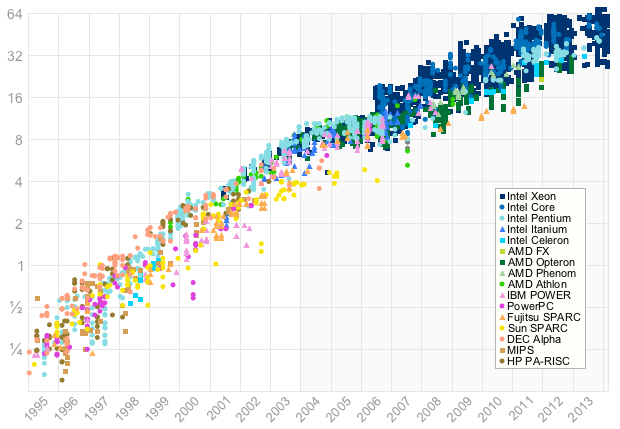
\includegraphics[width=\textwidth]{cpugrowth}
\caption{incremento nel tempo della capacità di elaborazione \cite{URL:cpuimage}. L'asse verticale impiega una scala logaritmica per visualizzare i \textit{benchmark} normalizzati ottenuti 
nell'elaborazione di interi con singolo \textit{thread}. È possibile notare nella prima parte un incremento costante del 50\%, che diminuisce dal 2004 assestandosi al 21\%.}
\label{cpuinc}
\end{figure}

Analogo ed essenziale è stato l’aumento della capacità di memorizzazione dei dispositivi in commercio. Negli anni ‘90 i computer possedevano \textit{hard disk} con dimensione media di 120 MB 
e tale capacità sembrava ampiamente sufficiente per le esigenze di chi allora li utilizzava; nel 2001 sono arrivati ad avere una capacità media di 40 GB \cite{URL:storagegrowth}; 
nel 2014, vengono venduti a prezzi modici \textit{hard disk} di dimensione pari a 4 TB. Quello che stupisce non è l’incremento delle capacità di questi supporti, facilmente prevedibile 
osservando quanto accaduto per i processori, ma la facilità con cui questi dispositivi possano essere occupati in breve tempo, proprio a causa della enorme mole di dati a disposizione 
degli utenti.

\begin{figure}[ht]
\centering
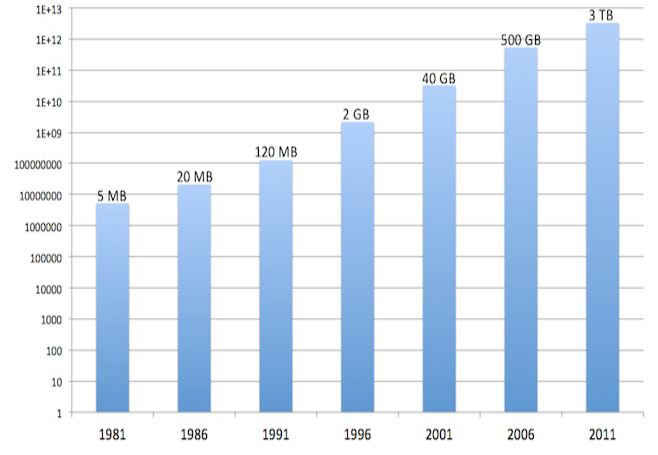
\includegraphics[width=\textwidth]{harddisk}
\caption{incremento nel tempo della capacità di memorizzazione \cite{URL:storagegrowth}.}
\end{figure}

\begin{figure}[ht]
\centering
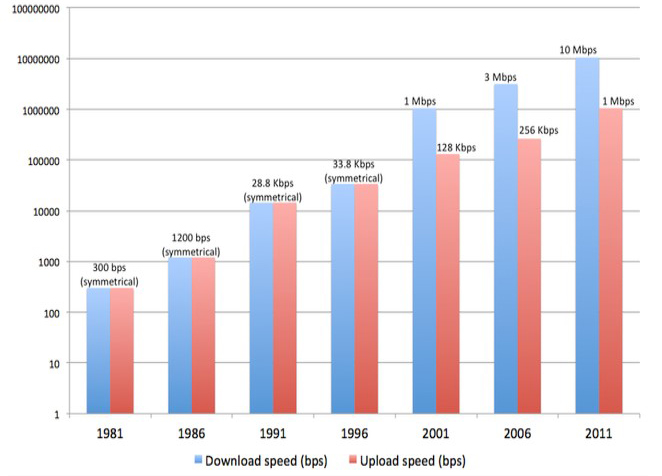
\includegraphics[width=\textwidth]{updown}
\caption{incremento nel tempo delle velocità di \textit{download} ed \textit{upload} \cite{URL:storagegrowth}.}
\end{figure}

Per condividere tutte queste informazioni su Internet gli utenti hanno necessitato di una infrastruttura che fornisse loro un’adeguata velocità di connessione. Anche in questo caso 
lo sviluppo tecnologico ha fornito loro degli strumenti adeguati. Uno studio condotto da Jakob Nielsen nel 1998 \cite{URL:nielsenlaw} ha portato alla 
formulazione di una legge, simile a quella di Moore, che descrivesse bene il tasso di crescita della velocità di connessione, di seguito riportata nella forma sintetica:

\begin{lstlisting}[breaklines]
Users' bandwidth grows by 50% per year (10% less than Moore’s Law).
\end{lstlisting}

I dati raccolti negli ultimi 15 anni confermano la legge e nel 2013 si è raggiunta una velocità di connessione media di 58 Mbps, una larghezza di banda che consente di condividere
contenuti a ritmi elevatissimi.

Infine, la diffusione di smartphone e di altri dispositivi portabili ha dato agli utenti la possibilità di condividere contenuti ovunque essi si trovino. Il risultato è stato un 
aumento dell’utilizzo giornaliero medio di Internet, che è passato dai 46 min/giorno del 2002 alle 4 ore/giorno del 2012 \cite{URL:increaseusage}.

L’incremento delle capacità dei computer, la diffusione di nuovi dispositivi mobili e la creazione di una rete che li connettesse tutti in modo veloce sono espressioni di un’equazione 
che ha come unica e scontata soluzione i \textit{big data}.


\section{Sorgenti di nuovi dati}

Le sorgenti di informazioni che producono \textit{big data} sono molte più di quelle facilmente immaginabili. Non siamo pienamente coscienti di quanto succede intorno a noi poiché i dispositivi 
tecnologici sono diventati parte della nostra quotidianità: li utilizziamo in modo trasparente, senza renderci conto della loro presenza. Il risultato è che generiamo e consumiamo 
continuamente dati, ma non ce ne accorgiamo.

Gli utenti del web sono raramente consci di produrre nuovi dati con le loro operazioni: il più delle volte, infatti, non sono consapevoli dei processi che vengono avviati in \textit{client} 
sparsi nel mondo in risposta alle loro azioni. Realizzano di stare generando nuove informazioni, invece, pubblicando video su YouTube (si stima che ogni minuto vengano caricate 
100 ore di contenuti \cite{URL:mediastats2014}), creando nuove pagine web o caricando i loro file su servizi di \textit{cloud storage} come Dropbox o Google Drive. 
Non lo sono pienamente, al contrario, quando effettuano ricerche su motori di ricerca, comprano oggetti \textit{online}, avviano un \textit{download} o cambiano 
canale sul televisore. Ogni azione che coinvolge l’utilizzo di Internet produce nuovi dati, che vengono conservati ed analizzati, con insidie latenti per la privacy degli 
utenti \cite{privacy1} \cite{privacy2}.

Poiché i piccoli circuiti integrati sono diventati economici, è stato possibile aggiungerli ad ogni oggetto per dotarlo di una componente di intelligenza. Perfino le reti ferroviarie 
sono provviste di sensori, che permettono di monitorare traffico, condizioni meteorologiche, stato delle spedizioni e condizioni dei binari, in modo da prevedere ed evitare incidenti. 
Con questi dispositivi vengono costantemente raccolti voluminosi dati ambientali, finanziari, medici e di sorveglianza in tutto il mondo, ma contribuiscono a produrre molte informazioni
anche giornali, riviste, sms, telefonate e sensori integrati nei dispositivi, come gli smartphone.

Una delle più grandi fonti di informazioni, tuttavia, si è costituita solo negli ultimi anni ed è di interesse specifico per questo lavoro: i \textit{social network}. L’espansione capillare 
di questi siti web ha portato ad un aumento sensibile della mole di dati prodotti dall’uomo. A fronte dell’importanza di tali siti web per questo studio, si ritiene opportuno darne 
una descrizione più approfondita.

\subsection{Social network}
I \textit{social network} sono siti che permettono agli utenti di costituire una rete di connessioni virtuali con altri individui, che siano amici o sconosciuti, e di restare in contatto con 
loro. Ciò che invoglia le persone ad utilizzarli è la facilità con cui essi potranno condividere i propri contenuti con i membri della loro rete. Tali contenuti sono spesso messaggi 
pubblici o privati, video, foto e notizie personali: nuove informazioni che, nel complesso, costituiranno \textit{big data}.

I tanti \textit{social network} attualmente \textit{online} si differenziano principalmente per il \textit{target} di utenti cui si rivolgono e per la tipologia di contenuti che tendenzialmente raccolgono. 
Tutti condividono, però, alcune caratteristiche peculiari. Dinamiche condivise sono la registrazione di un profilo con le informazioni personali, la condivisione di nuovi elementi, 
l’instaurazione di nuovi legami e la visualizzazione di contenuti appartenenti ad altri individui.

Elencare i più famosi \textit{social network} e descriverne le caratteristiche principali non è necessario ai fini di questo lavoro. Risulta anche inutile riportare tante statistiche 
riguardanti questi siti, poiché la maggior parte di esse non sarà più valida nel momento in cui qualcuno le leggerà. Per tale motivo ci si limiterà esclusivamente a descrivere 
Facebook e Twitter, due dei principali \textit{social network} contemporanei, che sono stati oggetti di studio.

Facebook, fondato nel 2004, rappresenta il più fulgido esempio di \textit{social network} e si può affermare che esso stesso abbia contribuito alla definizione dei canoni propri di questi 
siti. Ogni iscritto a Facebook possiede un diario personale, con visibilità pubblica o limitata, sul quale può pubblicare aggiornamenti di stato, foto, video, note e link a pagine web. 
Chi vuole ha facoltà di aggiungere, tra le sue informazioni personali, dettagli inerenti luogo e data di nascita, preferenze musicali, situazione sentimentale, orientamento politico 
o religioso, ecc. Il lato \textit{social} di Facebook consiste nella possibilità di aggiungere nuovi amici con cui condividere tutti o alcuni dei suddetti contenuti. Negli anni successivi sono 
state introdotte altre novità che hanno decretato il successo del \textit{social network}, ad esempio la possibilità di utilizzare applicazioni, chattare con gli amici o creare gruppi di 
interesse, pagine (spesso utilizzate per attività commerciali) ed eventi. Facebook ha conosciuto una rapida espansione fino a diventare il secondo sito più visitato al mondo, secondo 
solo a Google. Gli utenti attivi mensilmente su Facebook ammontavano a un milione nel 2004, a 145 milioni nel 2008 ed a 1,23 miliardi nel 
2013 \cite{URL:facebookstats} (approssimativamente 1/7 degli abitanti del pianeta). Si stima che, nel 2012, ogni minuto 
venissero inviati 510000 commenti, 293000 aggiornamenti di stato e 136000 foto \cite{URL:mediastats2012}.

Più modesti, ma non per questo meno straordinari, sono i numeri che gravitano attorno a Twitter, nato nel 2006 ed attualmente in settima posizione nella classifica dei siti più 
visitati al mondo, subito dopo Wikipedia e prima di Amazon \cite{URL:alexatop}. Le dinamiche di interazione con il \textit{social network} sono più limitate rispetto a quelle 
di Facebook. Gli utenti di Twitter - sono stimati 255 milioni di utenti attivi mensilmente \cite{URL:mediastats2014} - 
utilizzano il sito principalmente per inviare messaggi, detti \textit{tweet}, aventi una lunghezza massima di 140 caratteri. Sebbene sia possibile configurare la visibilità dei propri messaggi, 
Twitter viene usato solitamente senza filtri di sorta, lasciando visibili al mondo intero i propri \textit{tweet}, diversamente da quanto avviene normalmente con Facebook, ove la visibilità è 
generalmente limitata agli amici. Nei \textit{tweet} spesso vengono menzionati altri utenti o vengono inseriti dei \textit{tag}, detti \textit{hashtag}, che specificano il contenuto del messaggio o lo 
arricchiscono con informazioni o stati d’animo. Gli \textit{hashtag} vengono usati per permettere al sistema di individuare e mostrare le tendenze che si delineano tra i circa 500 milioni 
di messaggi giornalieri \cite{URL:mediastats2014}.

Il risultato di queste incessanti attività è che ogni giorno Facebook produce oltre dieci TB di nuovi dati e Twitter altri sette. Se a questi si aggiungono i dati generati anche
sugli altri \textit{social network} allora risulta evidente quanto sia abbondante la sorgente di nuove informazioni. Con questi ritmi non sembrano esagerate le stime del volume di dati 
memorizzati nel mondo: 800000 PB nel 2000, 161 EB nel 2006, 35 ZB stimati per il 2020 \cite{ibm:def1} \cite{idcexp}.


\section{Opportunità di business}
\label{par:money}

Per le sfide che impongono, potrebbe sembrare che i \textit{big data} siano un problema per chi si trova a doverli trattare. In realtà, se sapientemente elaborati, essi costituiscono 
un’occasione per considerevoli guadagni. Non a caso, infatti, le aziende che dispongono di più informazioni personali detengono più potere e ricchezza (Google, Amazon, eBay, 
Facebook, etc) \cite{URL:top30ent} e non deve stupire il fatto che sempre più imprese provino a comprare da loro dati con cui profilare gli individui.

Sembra ormai assodata l’uguaglianza tra \textit{big data} e \textit{big power}. In verità \textit{big data} è sinonimo di \textit{big latent power}, poiché questi dati richiedono un processo accurato di elaborazione,
al fine di estrarre conoscenza utile per un dominio applicativo o esigenze di mercato.

Il motivo per cui i dati rappresentano una così importante fonte di guadagno si può facilmente immaginare: conoscere abitudini e preferenze delle persone significa poter proporre 
loro pubblicità mirate oppure prevedere il loro comportamento ed agire di conseguenza. Emblematico è il caso di un \textit{discount} che nel 2002 ha assunto uno statistico per provare a 
predire quali consumatrici fossero incinte, al fine di pubblicizzare prodotti specifici per i neonati. I proprietari erano convinti, infatti, che identificando una donna nel secondo 
trimestre della gravidanza avrebbero avuto modo di fidelizzarla per anni, prima vendendole pannolini, poi cereali, libri e DVD \cite{URL:fidelity}.

La conoscenza degli utenti, comunque, è utilizzabile in diversi altri modi oltre al marketing personalizzato, ad esempio per dotare i sistemi di interfacce grafiche personalizzate 
per ogni individuo, per guidare scelte operative (quante scorte avere in magazzino di un determinato prodotto), campagne politiche, ecc.

Ciò che succede è che sempre più organizzazioni hanno accesso ad un gran numero di informazioni (pagine web, file di \textit{log}, \textit{click-stream data}, documenti, sensori), ma non sanno come
valorizzarle. Una indagine dell’IBM \cite{ibm:def1} ha riscontrato come oltre metà dei \textit{business leader} sentono di non avere gli strumenti adeguati per comprendere ciò che è necessario 
per la loro attività. Per tali ragioni, sempre più spesso, non sanno se conviene investire denaro e conservare questi dati (ammesso che abbiano i mezzi per farlo), nonostante siano
sempre più numerosi gli strumenti che permettono di analizzarli per ottenere una visione più chiara del proprio business, dei clienti e del mercato.

Un altro problema che gli imprenditori devono affrontare è quello della sempre minore longevità dei dati. Ad oggi, infatti, non siamo più in grado di leggere gli \textit{8-track tape}, 
i \textit{floppy disk} ed i VHS, rispettivamente di 30, 20 e 10 anni fa. La durata media della vita dei dispositivi di memorizzazione è sempre più breve e gli strumenti correlati diventano 
obsoleti. Un \textit{hard drive} è progettato per durare 5 anni, un nastro magnetico 10 e CD/DVD approssimativamente 20, sebbene già ora inizino ad essere impiegati sempre meno, in favore 
dei \textit{blu-ray disc}. Ci troviamo di fronte ad un paradosso per il quale le capacità di produrre e memorizzare dati aumentano, ma la capacità di conservarli nel tempo diminuisce. 
Moltissime aziende, infatti, hanno dovuto trascrivere i loro dati su nuovi supporti con una cadenza di 10-20 anni. Il fenomeno a cui si assiste è la crescita, per dimensione e 
complessità, dei dati a disposizione di una azienda a discapito della capacità di poterli analizzare. Col passare del tempo questo \textit{gap} sembra aumentare in modo incontrollato: 
gli imprenditori che si doteranno di strumenti per colmare questo divario sono quelli che controlleranno in futuro il mercato.

Analizzare i \textit{big data} prodotti dai propri utenti, tuttavia, non è l’unico modo che gli \textit{entrepreneur} hanno a disposizione per monetizzare. Diverse sono le aziende, infatti, 
specializzate nello sviluppo di tecnologie per l’analisi di questi dati che vengono poi noleggiate a terzi per ottenere importanti guadagni. Anche senza possedere \textit{big data}, 
pertanto, gli imprenditori possono sviluppare dei servizi da vendere a chi ne dispone. Tali servizi possono riguardare infrastrutture per la loro memorizzazione o tecnologie 
per poterli elaborare efficientemente, finanche in tempo reale. Diverse sono le redditizie piattaforme sviluppate da colossi dell’IT ed offerte alle imprese; alcune delle 
principali sono di proprietà di Amazon, Google, IBM e Microsoft. Tralasciando queste tecnologie, diverse aziende vendono strumenti per l’analisi ed infrastrutture.


\section{Criticità nella gestione}
\label{par:crit}

La natura dei \textit{big data}, come è stato anticipato, solleva diverse problematiche risolubili solo con particolari tecnologie. Ogni azienda possiede un numero di informazioni 
variabile ed è interessata ad elaborare i propri dati per conseguire uno specifico obiettivo, pertanto i processi che essi subiranno cambieranno in ogni contesto. È possibile, 
tuttavia, individuare due criticità comuni a tutti i casi d’uso: l’elaborazione e la memorizzazione dei dati.

Nel momento in cui si deve progettare un sistema avente come obiettivo l’analisi di grandi moli di informazioni bisogna decidere con quali modalità sarà eseguita la computazione 
e in che modo saranno memorizzati i dati. I criteri che dovrebbero orientare il progettista verso una scelta consona sono due: la natura delle operazioni che si desidera effettuare 
e la loro frequenza.

In base alle esigenze proprie del dominio, bisognerà trovare perciò la soluzione più adatta a risolvere i quattro problemi tipici della gestione di \textit{big data}: come avviene 
l’elaborazione e come la memorizzazione, dove avviene l’elaborazione e dove la memorizzazione.

Nel corso dei capitoli seguenti saranno presentati nel dettaglio dei \textit{framework} e degli strumenti progettati per risolvere questi problemi e che vengono tuttora frequentemente
impiegati in molteplici scenari; adesso ci si limiterà a presentare sommariamente, per ogni problema, i due principali approcci tra cui scegliere.

Il primo problema riguarda come effettuare le operazioni sui dati. Questa scelta ha anche un impatto diretto sul paradigma di programmazione adottato in fase di scrittura 
del codice del programma preposto all’elaborazione dei dati. È possibile seguire un approccio classico ed elaborare i dati in modo centralizzato, su un unico \textit{client}, 
oppure cercare una soluzione più scalabile, optando per una modalità di elaborazione distribuita tra più nodi di una rete. Questo secondo approccio è quello più adottato
e, per tale motivo, i \textit{framework} che consentono una ripartizione automatica del carico di lavoro tra computer interconnessi hanno conosciuto una rapida evoluzione. Un esempio
è offerto da Apache Hadoop, che sarà approfondito nel capitolo successivo.

Per quanto concerne le modalità di memorizzazione delle informazioni, è possibile scegliere tra la consolidata soluzione offerta dai database relazionali oppure scegliere 
sistemi innovativi per conservare i dati. Nel corso del capitolo \ref{chap:nosql} sarà effettuato uno studio comparativo dei database NoSQL, una nuova tipologia di database che meglio si 
adatta a gestire \textit{big data}.

Le soluzioni al problema riguardante l’ubicazione del processo di elaborazione sono riconducibili a due tipologie principali: effettuare la computazione in locale su uno o
più \textit{client} propri oppure percorrere la via del \textit{cloud computing}, delegando l’elaborazione a \textit{client} remoti. Come detto nel paragrafo precedente, diverse aziende come Amazon e
Google offrono dei servizi con cui è possibile elaborare efficientemente grandi moli di dati. In seguito verrà dimostrato come essi costituiscano un’opzione valida ed 
economicamente vantaggiosa rispetto all’effettuare il processo di elaborazione su macchine in locale.

Le opzioni appena illustrate per risolvere il problema dell’elaborazione sono anche valide per quello della memorizzazione. È possibile conservare i dati su \textit{client} propri 
in locale oppure optare per il \textit{cloud storage}, trasferendo i propri file in rete. Anche per questo scopo è possibile trovare \textit{online} servizi di noleggio di spazio virtuale 
ove caricare i propri dati e renderli disponibili in qualunque momento e da qualunque parte del globo.

Tutte le varie possibilità presentate offrono ai progettisti ampia libertà di scelta. Essi potranno propendere per una architettura interamente \textit{cloud} oppure per soluzioni 
ibride, che impiegano servizi remoti solo per soddisfare alcune necessità, delegando ai propri \textit{client} il resto delle operazioni. 

Progettare correttamente la struttura del sistema risulta fondamentale quando vengono elaborati \textit{big data}, poiché è alta la probabilità di incappare in \textit{bottleneck} che potrebbero
far degradare le performance del sistema. Ulteriore attenzione va posta se si adoperano soluzioni \textit{cloud}, poiché vanno studiati attentamente i costi di questi servizi al fine
di valutare l’effettiva economicità dell’opzione.

\chapter{Elaborazione distribuita: Apache Hadoop}
\label{chap:hadoop}

\section{Descrizione del framework}

Un punto di svolta fondamentale nello sviluppo di tecnologie orientate ai \textit{big data} è stata la pubblicazione, ad opera di Google, di alcuni articoli in cui venivano illustrati i 
principi di funzionamento di alcuni strumenti sviluppati ed utilizzati dal colosso per far fronte alle proprie gravose esigenze. Il \textit{paper} sul Google File System del 
2003 \cite{google:filesystem} e quello su MapReduce del 2004 \cite{google:mapreduce}, più degli altri, hanno radicalmente cambiato il modo di pensare ai dati ed hanno avviato 
lo sviluppo di molte nuove tecnologie, tra cui Hadoop \cite{hadoop}. 

Hadoop è un progetto \textit{top-level} della Apache Software Foundation, scritto in Java da una community globale di contributori. Lo sviluppo del \textit{framework} è cominciato nel 2004 come 
sotto-progetto di Lucene, una libreria per l’\textit{information retrieval}, da cui poi si è distaccato per divenire un progetto a sé stante. Hadoop ha avuto un’importante evoluzione dal
2005, sotto la spinta di Yahoo!, interessato a realizzare una tecnologia che potesse competere con quella sviluppata da Google. Nell’articolo del 2004 viene descritto MapReduce,
un modello di programmazione ed un omonimo \textit{framework} scritto in C++ progettati per eseguire in parallelo programmi su \textit{cluster} di computer. Il \textit{framework} di Google, di cui Hadoop 
è una riproduzione \textit{open-source}, si preoccupa di distribuire la computazione tra i nodi del \textit{cluster}, gestire i malfunzionamenti delle macchine, bilanciare i carichi di lavoro ed 
accorpare i risultati prodotti da ciascun nodo prima di restituirli in output all’utente. In questa maniera uno sviluppatore può concentrarsi sulla scrittura del codice del 
proprio programma, anche senza avere esperienza di computazione parallela, poiché essa sarà gestita automaticamente dal \textit{framework}. Il codice scritto, che deve aderire al modello 
di programmazione MapReduce (descritto nel dettaglio nel paragrafo \ref{par:hadoopmodel}), risulta lineare, poiché non contiene sezioni orientate a gestire meccanismi di parallelizzazione o 
recupero da situazioni di errore. 

In questa maniera Hadoop diventa lo strumento ideale, talvolta l’unica opzione possibile, per elaborare grandi moli di dati, perché permette di ripartire pesanti carichi di 
lavoro tra tante macchine di un \textit{cluster}, ciascuna delle quali processa solo una ridotta frazione dei dati di input. Per tal motivo, moltissime 
aziende \cite{URL:usinghadoop} che trattano \textit{big data}, quali Yahoo!, Facebook, Twitter, eBay, LinkedIn e Spotify, impiegano \textit{cluster} con Hadoop per effettuare 
l’elaborazione dei propri dati. Intorno ad Hadoop si sono poi sviluppati numerosi altri progetti, tra cui HBase, Pig, Hive e Spark, che vengono per convenzione inclusi nella
“piattaforma Hadoop”. Questi progetti, generalmente, utilizzano Hadoop nel loro \textit{core} per aggiungergli delle caratteristiche o realizzare tecnologie più complesse, come database 
o strumenti di analisi. 

Nella sua versione iniziale Hadoop era progettato per l’elaborazione \textit{batch} dei dati, ma ora ci sono diversi servizi che consentono di adoperarlo in applicazioni \textit{real-time} 
(\textit{stream-processing}, \textit{real-time} \textit{query}, ecc.). 

I moduli principali che compongono il \textit{framework} dell’ultima versione (2.5.0) sono: Hadoop Common, una raccolta di strumenti impiegati da diversi moduli, Hadoop Distributed 
File System (HDFS), il \textit{file system} presentato nel dettaglio in seguito, Hadoop YARN, un \textit{framework} per il \textit{job scheduling} e la gestione delle risorse del \textit{cluster} e Hadoop MapReduce,
il sistema basato su YARN per elaborare in parallelo grandi \textit{dataset}. 

Nonostante sempre più strumenti vengano sviluppati per elaborare in parallelo i dati, Hadoop rimane una tecnologia largamente impiegata nelle imprese dell’IT. A conferma di 
quanto detto, diverse sono le importanti aziende che offrono \textit{software} o servizi basati sul \textit{framework}: alcuni esempi sono Cloudera, MapR e Hortonworks, aziende specializzate 
nello sviluppo di piattaforme e strumenti per l’analisi di \textit{big data}.

Nei paragrafi seguenti saranno descritti l’Hadoop Distributed File System ed il modello di programmazione MapReduce, essenziali per comprendere i principi di funzionamento del \textit{framework}.


\section{Hadoop Distributed File System}
\label{chap:hdfs}

Una componente essenziale del \textit{framework} è il \textit{file system} che tutti i nodi del \textit{cluster} utilizzano: l’Hadoop Distributed File System (HDFS).

La necessità di sviluppare un \textit{file system} specifico per Hadoop derivava da due esigenze avvertite, sin dalle fasi iniziali dello sviluppo, dai contributori del progetto. Il primo 
problema da risolvere era causato dalla natura distribuita del \textit{framework}: ogni nodo del \textit{cluster}, infatti, per eseguire i compiti assegnati, doveva poter accedere ai dati di input 
del programma. La seconda problematica, invece, era legata alla tipologia di questi dati di input: \textit{big data}, non memorizzabili fisicamente su una solo macchina, coerentemente con 
la definizione data nel paragrafo \ref{par:defbigdata}. Replicare i \textit{dataset} su ogni nodo, pertanto, risultava impossibile.

L’Hadoop Distributed File System risolve questi ed altri problemi adoperando soluzioni architetturali già presenti in altri \textit{file system} distribuiti ed ignorando alcuni vincoli POSIX 
per ragioni di efficienza, similmente al Google File System (GFS). Una assunzione che viene fatta, ad esempio, è che i dati del \textit{cluster} siano soggetti a \textit{batch processing} e pertanto
il modello adottato è di tipo \textit{write-once-read-many}. Per tale motivo, una volta creati, i file non possono essere modificati (nel GFS, invece, è possibile eseguire operazioni atomiche 
di \textit{append}): questo, sebbene rappresenti un grande limite, consente di ottenere un elevato \textit{throughput}.

L’HDFS gestisce i file in modo gerarchico, come un \textit{file system} tradizionale, utilizzando cartelle e \textit{path}, con la differenza che i dati non vengono memorizzati fisicamente in un unico
 luogo, ma vengono ripartiti tra i nodi di un \textit{cluster}. I file, infatti, vengono suddivisi in \textit{chunk} di 64 MB (l’ultimo \textit{chunk} può avere dimensione inferiore) e distribuiti tra i nodi, 
 che, in questo modo, si dividono l’onere di conservare grandi moli di dati. Il \textit{file system} è progettato per essere avviato su grandi \textit{cluster} con \textit{commodity hardware}, dove i
 malfunzionamenti non sono un caso, quanto la norma (\textit{crash} delle macchine, rottura dei \textit{drive}, errori di rete, ecc.). Per tale motivo, al fine di garantire sempre la disponibilità 
 dei dati, i \textit{chunk} vengono replicati (il fattore di replicazione di \textit{default} è tre, ma è configurabile).

A livello architetturale l’HDFS presenta una struttura \textit{master}/\textit{slave}, illustrata in figura \ref{hdfsimage}. Un unico nodo \textit{master}, il NameNode, si preoccupa di gestire il \textit{file system}, conservando 
l’elenco dei file memorizzati e tenendo traccia della loro ubicazione nel \textit{cluster} attraverso metadati. Tutti gli altri nodi \textit{slave} del \textit{cluster}, invece, ricoprono il ruolo di DataNode 
e conservano i \textit{chunk} che sono loro assegnati dal NameNode. Quest’ultimo, conoscendo la locazione dei \textit{chunk}, può indirizzare le richieste del \textit{client} ai DataNode opportuni, che si 
occuperanno di leggere i dati ed inviarli al programma che li consumerà. Il NameNode si preoccupa, inoltre, di eseguire operazioni quali la rinomina o la cancellazione dei file, 
ma anche di verificare che i \textit{chunk} siano integri (attraverso il \textit{checksum}) e che siano sufficientemente replicati (in caso negativo avvia la loro copia su nuovi DataNode).

\begin{figure}[ht]
\centering
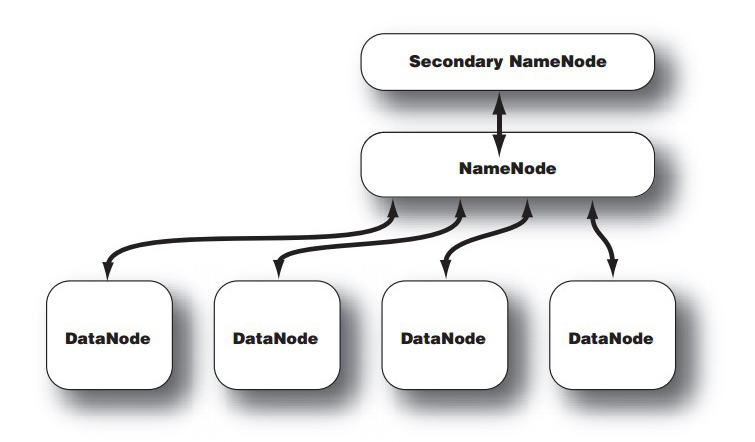
\includegraphics[width=\textwidth]{hdfsimg}
\caption{architettura dell'HDFS \cite{hadoop}.}
\label{hdfsimage}
\end{figure}

Diversi accorgimenti permettono al NameNode di mantenere un indice dei \textit{chunk} sempre aggiornato per fornire dati consistenti a chi legge dal \textit{file system}. Esso conserva in memoria, 
innanzitutto, un file contenente le proprietà del sistema ed il \textit{mapping} tra i blocchi dei file ed i nodi del \textit{cluster}. Tale file, detto FsImage, viene periodicamente serializzato 
ed occupa poco spazio (un NameNode con 4 GB di RAM supporta un numero enorme di file e \textit{directory}). Al suo avvio, il NameNode carica l’ultima FsImage ed interroga tutti i DataNode
del \textit{cluster} che gli forniscono una risposta, detta BlockReport, contenente l’elenco dei \textit{chunk} da loro attualmente conservati; combinando le informazioni ottenute, il nodo \textit{master} 
ottiene una rappresentazione generale del sistema e provvede a verificare che ogni file sia aggiornato e sufficientemente replicato. Tutte le azioni eseguite dal NameNode sul 
\textit{file system}, inoltre, vengono memorizzate e replicate in un file di \textit{log}, detto EditLog, che consente, in caso di fallimento del nodo \textit{master}, di ripristinare al suo riavvio l’ultima 
configurazione del \textit{file system}. Il nodo \textit{master}, infatti, ricarica l’ultima FsImage e riesegue su di essa le ultime operazioni andate perdute. Per tale motivo, una volta serializzata
una nuova FsImage, l’EditLog può essere svuotato, poiché le ultime modifiche sono conservate nell’ultima immagine del sistema.

L’HDFS non supporta gli \textit{snapshot} per memorizzare una copia dei dati ad un certo istante temporale - il GFS, invece, beneficia di questa funzionalità – e non dispone di un meccanismo 
per riavviare automaticamente il NameNode in caso di malfunzionamenti. Quest’ultimo, inoltre, rappresenta un \textit{single-point-of-failure} del sistema, poiché è l’unico a poter eseguire 
operazioni sul \textit{file system}. A fronte di questi svantaggi, tuttavia, l’HDFS presenta altri punti di forza, tra cui una indiscutibile semplicità di accesso. Esso può essere utilizzato
dalle applicazioni in diverse maniere; espone infatti una API Java ed un \textit{wrapper} in C di tale API, consente la navigazione tramite browser mediante il protocollo HTTP e la \textit{shell} 
presenta la maggior parte dei comandi tradizionali riguardanti i file con semantica intuitiva. Un’altra interessante caratteristica del \textit{framework} riguarda la capacità di suddividere 
in modo ottimale le repliche dei \textit{chunk} tra i DataNode per ottimizzare le performance in fase di lettura. L’HDFS, infatti, in linea col principio secondo cui “\textit{moving computation 
is cheaper than moving data}”, cerca di minimizzare lo spostamento di dati sulla rete, distribuendo in modo omogeneo i blocchi di file tra i vari \textit{rack} del \textit{cluster}, per consentire 
ai \textit{client} di avere sempre a brevi distanze dei nodi contenenti le informazioni a loro necessarie.


\section{Modello di programmazione MapReduce}
\label{par:hadoopmodel}

In questo paragrafo vengono descritti i principi fondamentali del modello di programmazione MapReduce, alla base sia del \textit{framework} di Google, che di quello di Apache; per tale motivo, 
durante la descrizione, ci si riferirà indistintamente ai due prodotti, poiché le differenze che sussistono riguardano principalmente dettagli realizzativi e non strutturali.

Per semplificare il processo di elaborazione dei dati avvantaggiandosi del \textit{framework}, i programmi da eseguire sul \textit{cluster} devono essere costituiti da due operatori: \textit{map} e \textit{reduce}. 
Nonostante le tipologie di computazione da effettuare sui dati siano di natura diversa, la maggior parte di esse può essere realizzata impiegando queste due sole funzioni, come 
spiegato anche nell’introduzione di Google su MapReduce:

\begin{lstlisting}[breaklines]
We designed a new abstraction that allows us to express the simple computations we were trying to perform but hides the messy details of parallelization, fault-tolerance, data distribution and load balancing in a library. Our abstraction is inspired by the map and reduce primitives present in Lisp and many other functional languages. We realized that most of our computations involved applying a map operation to each logical "record" in our input in order to compute a set of intermediate key/value pairs, and then applying a reduce operation to all the values that shared the same key, in order to combine the derived data appropriately.
\end{lstlisting}

Un programma che implementa correttamente le funzioni \textit{map} e \textit{reduce} è in grado di essere eseguito dal \textit{framework} in modo distribuito: il programmatore può, perciò, concentrare la 
sua attenzione esclusivamente sulla scrittura di tali operatori.

La funzione \textit{map} riceve in input una coppia chiave/valore (K, V) e produce in output un insieme di coppie intermedie chiave/valore (I, P). Il \textit{framework} raggruppa automaticamente 
le coppie intermedie aventi stessa chiave I e inserisce tutti i corrispondenti valori P in una lista. La funzione \textit{reduce} riceve in input una di queste coppie (I, [P1, P2, P3, …]) 
generate dal \textit{framework} e produce un insieme, possibilmente ridotto, di tali valori. È possibile schematizzare le funzioni nel modo seguente:

\begin{lstlisting}[frame=single]
map (K, V) -> list(I, P)
reduce (I, list(P)) -> list(P)
\end{lstlisting}

I tipi delle chiavi e dei valori intermedi sono solitamente quelli supportati dal linguaggio di programmazione del \textit{framework}; generalmente sono sufficienti interi, \textit{double}, \textit{long} 
e stringhe per la maggior parte dei casi d’uso.

Il \textit{framework} assegna ai nodi del \textit{cluster} l’esecuzione di una o più funzioni \textit{map}/\textit{reduce} e ne raccoglie i risultati (per i dettagli sul funzionamento si rimanda al paragrafo successivo).
Ciascun nodo possiede il codice di entrambi gli operatori e, su richiesta del \textit{framework}, esegue la funzione che gli viene richiesta sui dati di input che riceve.

Per chiarire quanto appena spiegato viene presentato lo pseudo-codice delle funzioni \textit{map} e \textit{reduce} che si potrebbero scrivere per indicizzare un documento:

\begin{lstlisting}[frame=single]
map(int lineNumber, String line):
  for each word w in line:
    EmitIntermediate(w, 1);
\end{lstlisting}

\begin{lstlisting}[frame=single]
reduce(String w, List<Integer> values):
  Emit(w, length(values));
\end{lstlisting}

Il programma conta, per ogni parola, il numero di occorrenze nel documento. La funzione \textit{map} riceve in input una coppia avente per chiave un numero naturale rappresentante la 
riga i-esima del documento e per valore una stringa uguale alla riga i-esima. L’operatore itera su ogni parola w della riga e produce in output una coppia (w, 1), a significare 
che la parola w è stata incontrata una volta. Al termine dell’esecuzione di tutte le funzioni \textit{map}, il \textit{framework} si occuperà di accorpare le coppie aventi stessa chiave prodotte 
dai vari nodi del \textit{cluster}: per ogni parola w del documento verrà creata una coppia avente come chiave w e come valore una lista dei valori intermedi a lei abbinati (in questo 
caso una lista di numeri 1, provenienti dalle funzioni \textit{map} eseguite su diversi nodi). Le coppie di input per la funzione \textit{reduce} saranno pertanto della forma (w, list(1, 1, …, 1)),
che si limiterà a controllare la dimensione della lista per restituire in output coppie del tipo (w, \#occorrenze). 

Le funzioni potrebbero essere schematizzate così:

\begin{lstlisting}[frame=single]
map (int, String) -> list(String, int)
reduce (String, list(int)) -> (String, int)
\end{lstlisting}

Come è possibile notare, il modello di programmazione MapReduce permette di scrivere semplici funzioni, delegando al \textit{framework} l’onere di gestire il calcolo in parallelo tra 
i nodi. Le funzioni \textit{map} e \textit{reduce} illustrate permettono di indicizzare agevolmente \textit{dataset} dell’ordine di PB, a patto di avere \textit{cluster} di dimensione appropriata.


\section{Principi di funzionamento del framework}

Nel corso degli anni Hadoop è stato protagonista di una grande evoluzione, che ha causato, talvolta, modifiche sostanziali al \textit{framework} nel passaggio da una versione all’altra. 
Sebbene il \textit{core} sia rimasto immutato, diverse altre componenti sono cambiate radicalmente. Per tale motivo, nell’illustrare i principi di funzionamento di Hadoop, sarà scelta una 
versione di riferimento, la 0.18. I componenti fondamentali di questa \textit{release} sono rimasti pressoché immutati fino alla versione 2 del \textit{framework}, quando sono state introdotte molte 
novità, tra cui YARN. 

Come si è potuto evincere, un \textit{cluster} di Hadoop è composto da diversi nodi, ciascuno dei quali ricopre uno specifico compito. Tali ruoli vengono assegnati alle macchine in fase 
di configurazione del \textit{cluster} dal manager del sistema, che deve avere pertanto una conoscenza profonda dell’architettura del \textit{framework}: una corretta configurazione, infatti, è 
essenziale per ottenere elevate prestazioni. Sebbene scrivere programmi secondo il modello MapReduce sia relativamente semplice, configurare correttamente il \textit{cluster} può risultare 
laborioso per chi si approccia al \textit{framework} per la prima volta. Per questo motivo sono stati sviluppati degli strumenti per effettuare automaticamente il \textit{tuning} dei parametri di 
configurazione (ad esempio Starfish) e \textit{file system} personalizzabili per eseguire il \textit{deploy} del \textit{cluster} (ad esempio quello offerto dalla Google Cloud Platform).

Eseguire un \textit{cluster} di Hadoop significa avviare su ciascun nodo uno o più \textit{daemon}, che specificano il ruolo del nodo nella rete. In generale, è possibile suddividere i \textit{daemon} in 
due classi: quelli di computazione e quelli di memorizzazione. I \textit{daemon} di computazione sono il JobTracker ed il TaskTracker, mentre quelli di memorizzazione sono il NameNode, 
il Secondary NameNode ed il DataNode.

\begin{figure}[ht]
\centering
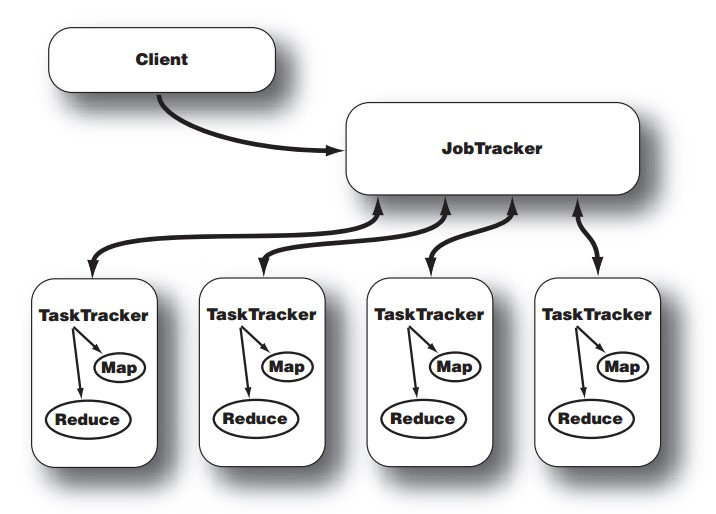
\includegraphics[width=\textwidth]{hadoopimg}
\caption{architettura del framework \cite{hadoop}.}
\label{hadoopclient}
\end{figure}

Il JobTracker è il punto di collegamento tra l’applicazione scritta dall’utente ed il \textit{framework} (come si può notare in figura \ref{hadoopclient}. Una volta inviato il proprio programma ad Hadoop, il JobTracker fissa un piano 
di esecuzione, assegna ai nodi disponibili dei \textit{task} da completare e si preoccupa di raccogliere e ridirezionare i risultati intermedi della computazione. Il \textit{daemon}, inoltre, 
controlla se i nodi lavoratori stiano correttamente funzionando interrogandoli periodicamente; se non riceve risposte da un nodo, il JobTracker assume che sia incappato in una 
situazione di errore e riassegna il \textit{task} ad un nuovo nodo inattivo. Nel \textit{cluster} vi è solo un JobTracker ed è tipicamente il \textit{master node} del \textit{cluster}. Esso rappresenta un 
\textit{single-point-of-failure} (con YARN, invece, il ResourceManager non è affetto da questa criticità). Generalmente non si eseguono TaskTracker sul nodo dove è in esecuzione il 
JobTracker al fine di non sovraccaricare ulteriormente la macchina e non incorrere in degradi di prestazioni.

Il TaskTracker è uno \textit{slave node} e si occupa di eseguire i \textit{task} \textit{map} e/o \textit{reduce} assegnatigli dal JobTracker, cui spedisce i risultati elaborati. Sebbene ci sia al più un solo 
\textit{daemon} TaskTracker in esecuzione su ogni nodo, ciascuno di essi può avviare istanze multiple della Java Virtual Machine, in modo da iniziare diversi \textit{task} in parallelo. Il 
TaskTracker, mentre svolge i compiti, informa periodicamente il JobTracker della sua attività.

Tra i \textit{daemon} di memorizzazione, NameNode e DataNode sono stati già esaustivamente descritti nel paragrafo sull’HDFS. Resta da analizzare il Secondary NameNode, sebbene il 
suo nome sia eloquente. Il ruolo di questo \textit{daemon}, infatti, è di assistenza al NameNode, che è un \textit{single-point-of-failure}, per monitorare lo stato del \textit{cluster}. Come per il 
NameNode, ogni \textit{cluster} ha un solo Secondary NameNode, che risiede generalmente su una macchina dedicata, senza altri \textit{daemon} in esecuzione. Esso non riceve in tempo reale 
aggiornamenti sulla situazione dell’HDFS, ma comunica ad intervalli configurabili con il NameNode per effettuare \textit{snapshot} dei suoi metadati. Le informazioni che il Secondary
NameNode memorizza possono aiutare a minimizzare i tempi di \textit{downtime} dovuti a fallimenti del NameNode principale, poiché è possibile, previo intervento manuale, promuovere il
Secondary NameNode a NameNode per riattivare il \textit{cluster}. Una rappresentazione di tutta l'architettura è fornita nella figura \ref{architecture}.

\begin{figure}[ht]
\centering
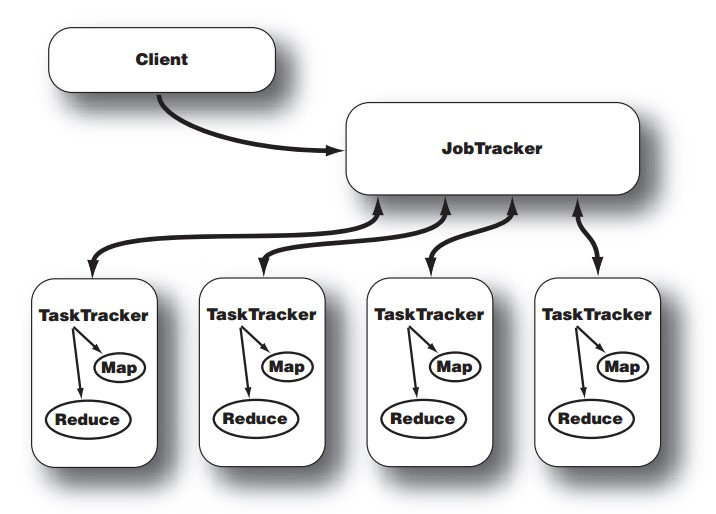
\includegraphics[width=\textwidth]{hadoopimg}
\caption{ubicazione dei \textit{daemon} nel \textit{cluster} \cite{hadoop}.}
\label{architecture}
\end{figure}

Su ciascun nodo \textit{slave} sono solitamente in esecuzione sia il DataNode che il TaskTracker per ripartire sia il carico di lavoro che quello di memorizzazione. Per ottenere buone
prestazioni, Hadoop è in grado di assegnare i \textit{task} di \textit{map} e \textit{reduce} in modo da sfruttare la località dei dati ed evitare inutili trasferimenti di informazioni nella rete. Il 
\textit{framework}, perciò, assegna i \textit{job} ai TaskTracker in esecuzione sulle macchine più vicine ai DataNode contenenti i dati di input necessari.


\subsection{Modalità di esecuzione}

Hadoop può essere eseguito in tre modalità differenti: locale, pseudo-distribuita e distribuita.

La modalità locale (\textit{standalone}), impiegata in \textit{default} da Hadoop, necessita di una sola macchina e non di un \textit{cluster}. In questa modalità non vengono avviati né i \textit{daemon} di Hadoop 
precedentemente illustrati né l’HDFS, poiché non ci sono forme di comunicazione tra i nodi: i dati ed il programma sono residenti sulla stessa macchina, che esegue un 
programma in modo tradizionale. Questa modalità è spesso impiegata in fase di sviluppo e di \textit{debug}, poiché permette di verificare la correttezza della logica di un’applicazione 
MapReduce, senza trattare con la complessità addizionale dovuta all’interazione con i \textit{daemon}.

Anche la modalità pseudo-distribuita richiede una sola macchina ed equivale ad eseguire un \textit{cluster} con un solo nodo. Su questo nodo vengono eseguiti tutti i \textit{daemon}, inclusi 
quelli dell’HDFS, perciò vi è comunicazione tra le istanze della Java Virtual Machine. Come per la modalità locale, anche quella pseudo-distribuita ha finalità di \textit{debug}. In 
modo particolare è utile per monitorare l’utilizzo della memoria, i problemi nei flussi di input/output dell’HDFS e, soprattutto, l’interazione tra i \textit{daemon}.

Vi è infine la modalità distribuita, impiegata quando la correttezza del programma è stata appurata mediante opportuni test con le altre modalità. In questa modalità diversi 
nodi formano un \textit{cluster} e su ciascuno vengono avviati i diversi \textit{daemon}, che interagiscono tra loro tramite SSH.


\subsection{Ottimizzazione delle performance}
\label{par:hadoopimprove}

Le informazioni finora fornite dovrebbero permettere una comprensione generale dell’architettura del \textit{framework}, ma ci sono alcuni altri elementi che vale la pena di approfondire.

Un punto cruciale nell’esecuzione di applicazioni MapReduce è il passaggio dal completamento dei \textit{job} di \textit{map} all’avvio di quelli di \textit{reduce}. Da quanto finora detto, sembrerebbe che 
sia Hadoop a gestire autonomamente questo momento della elaborazione. In effetti questo è il comportamento di \textit{default} del \textit{framework}, che, in modo trasparente all’utente, raccoglie 
in una lista i valori intermedi appartenenti ad una stessa chiave ed avvia funzioni di \textit{reduce} sulle coppie generate. In realtà lo sviluppatore può alterare le azioni che saranno 
eseguite al termine dei \textit{job} di \textit{map} per ottenere significativi aumenti nelle performance. Oltre alle classi Mapper e Reducer, che contengono, rispettivamente, le funzioni \textit{map} e 
\textit{reduce} e che devono tassativamente essere scritte, lo sviluppatore può definire un Combiner ed un Partitioner personalizzati. Se queste due classi non vengono configurate allora 
il \textit{framework} adopera quelle di \textit{default}, che impiegano funzioni di \textit{hash} per ripartire i dati in modo omogeno tra i nodi.

Il Combiner ha un ruolo simile al Reducer, poiché aggrega i valori delle coppie intermedie. Mentre il Reducer compatta le coppie provenienti da nodi differenti, il Combiner 
agisce su un singolo TaskTracker, prima che invii nel \textit{cluster} i risultati intermedi prodotti dalla funzione \textit{map}. Il Combiner ed il Reducer, in generale, possono aggregare dati 
in modo differente, secondo le esigenze specifiche del caso d’uso. Aggregare i dati su ciascun nodo, prima che vengano trasmessi nel \textit{cluster} può ridurre le operazioni di 
input/output migliorando il \textit{throughput} generale. A dimostrazione di ciò, viene ora arricchito il precedente esempio per l’indicizzazione di un documento introducendo un Combiner 
adatto, che sfrutta la proprietà associativa dell’addizione.

Il Mapper precedente resta invariato, mentre il Combiner aggiunto si limitar a sommare localmente il numero di occorrenze per ciascuna chiave (parola) prima di restituirlo in output. 
L’output del Mapper, perciò, non saranno più tante coppie (w$_{\mathrm{n}}$, 1), ma coppie del tipo (w$_{\mathrm{n}}$, \#occorrenze\_nella\_riga). A fronte di questo cambiamento, il codice del Reducer deve essere
lievemente modificato, poiché i valori associati ad una chiave non saranno più liste di 1, ma liste di interi probabilmente diversi tra loro. Il numero di occorrenze di una parola 
non sarà più dato dalla lunghezza della lista (un 1 per ogni match), ma dalla somma dei valori nella lista: 

\begin{lstlisting}[frame=single]
reduce(String w, List<Integer> values):
  int count = 0;
  for each value v in values:
    count = count + v;
  Emit(w, count);
\end{lstlisting}

Aggregando parzialmente le occorrenze in ogni TaskTracker, il numero di coppie immesse nella rete diminuisce drasticamente. Senza un Combiner, ogni riga del documento data in 
input ai Mapper produceva tante coppie quante le parole che conteneva; mediante il Combiner, invece, viene emessa una coppia in meno per ogni parola duplicata. Considerando che
un documento contiene moltissime parole duplicate, il numero di coppie trasferite diminuisce sensibilmente aumentando le performance generali.

Resta da approfondire il Partitioner, che ha il compito di ripartire le coppie prodotte dai Mapper - ed eventualmente aggregate dai Combiner - tra i nodi del \textit{cluster} che 
eseguiranno funzioni di \textit{reduce}. Il Partitioner di \textit{default} è l’HashPartitioner ed ha un ruolo fondamentale, poiché serve ad evitare \textit{bottleneck} nella fase conclusiva dell’applicazione:
se tutte le coppie intermedie, infatti, confluissero in un unico TaskTracker esso impiegherebbe una grande quantità di tempo per completare la fase di \textit{reduce}, nullificando i 
benefici guadagnati dell’elaborazione in parallelo nella fase di \textit{map}. Un Partioner preposto alla suddivisione di chiavi di tipo stringa, ad esempio, potrebbe suddividerle in base 
alla loro lunghezza o al loro primo carattere.

Altre due caratteristiche peculiari di Hadoop meritano un approfondimento: la \textbf{Streaming API} e la \textbf{DistributedCache}.

Hadoop può interagire con altri linguaggi attraverso una API generica, chiamata Streaming. Questa è particolarmente utile per la scrittura di semplici e brevi programmi MapReduce 
che possono essere sviluppati più facilmente in linguaggi di \textit{scripting} che non hanno bisogno di librerie Java. Hadoop Streaming interagisce con gli altri programmi usando il 
paradigma Unix: l’input arriva dallo \textit{STDIN} ed è direzionato in uscita verso lo \textit{STDOUT}. I comandi Unix funzionano con il \textit{framework}, che permette di impiegarli come funzioni \textit{map} 
o \textit{reduce}. In questo modo è possibile utilizzare, ad esempio, \textit{cut}, \textit{uniq}, \textit{wc} oppure \textit{script} in Python o PHP come parametri nella configurazione dei \textit{task} di Hadoop.

Il seguente esempio mostra un codice in Python della funzione \textit{map} per un \textit{job} di indicizzazione.

\begin{lstlisting}[frame=single]
#!/usr/bin/env python
     
import sys
     
for line in sys.stdin:
  line = line.strip()
  keys = line.split()
  for key in keys:
    value = 1
    print( "%s\t%d" % (key, value))
\end{lstlisting}

Una ultima caratteristica di Hadoop meritevole di essere illustrata è DistributedCache, un semplice ma utile meccanismo che consente di replicare automaticamente alcuni file 
tra tutti i nodi del \textit{cluster}. DistributedCache viene solitamente impiegato per fornire, spesso all’accensione, tutte le macchine del \textit{cluster} di file contenenti “dati di \textit{background}”, 
spesso richiesti dai Mapper. Può essere utilizzato, ad esempio, per distribuire file di configurazione, \textit{script} o documenti contenenti metadati. Nell’ormai noto esempio di indicizzazione 
del testo, ad esempio, la funzione di \textit{map} potrebbe necessitare di un \textit{tokenizer} per dividere una stringa in parole. Se il \textit{tokenizer} scelto fosse incluso in una libreria esterna, 
ad esempio, essa potrebbe essere distribuita tra tutti i nodi del \textit{cluster} tramite la funzionalità di DistributedCache. Tutte le funzioni \textit{map} potrebbero, pertanto, utilizzare quella 
libreria, perché certamente presente sul nodo corrente.

\chapter{Memorizzazione flessibile: database NoSQL}
\label{chap:nosql}

\section{Origini delle tecnologie}

Memorizzare negligentemente \textit{big data} è il presupposto fondamentale per poterli in seguito elaborare efficientemente. Come detto nel secondo capitolo, il problema che sorge
in fase di memorizzazione riguarda non soltanto lo spazio fisico che essi richiedono - col passare del tempo gli \textit{hard disk} diventano sempre più capienti ed economici - ma 
anche le modalità con cui essi vengono archiviati. Una scelta progettuale sbagliata, infatti, può comportare una incapacità di recuperare questi dati velocemente, causando 
problemi di entità variabile col contesto d’uso (si pensi alla criticità nei sistemi \textit{real-time} o a \textit{bottleneck} in fase di lettura). Quando bisogna trattate \textit{big data} è richiesto 
un consistente sforzo ingegneristico per sviluppare \textit{ex novo} soluzioni che ripartiscano l’onere di memorizzazione tra diverse macchine, in un modo simile a quanto illustrato 
con l’Hadoop File System nel capitolo \ref{chap:hdfs}. Infatti, sebbene sia facile aumentare la capacità di memorizzare dati comprando nuovi \textit{drive}, risulta comunque impensabile concentrare
tutto questo potenziale su un unico \textit{client}.

L’esigenza di ripartire il carico di lavoro senza degradare nelle performance ha reso inadatti i database tradizionali, che utilizzano il modello relazionale per la strutturazione
dei dati. Quando questi database sono stati progettati negli anni ‘70, infatti, Internet era ancora in uno stato embrionale: non esistevano \textit{social network}, smartphone e \textit{big data}
e, soprattutto, non si avvertiva l’esigenza di sviluppare sistemi che potessero scalare. Ma il \textit{Web 2.0} ha generato nuovi bisogni che i database NoSQL hanno provato a soddisfare.

Il termine ``\textit{NoSQL}'' include un’ampia gamma di tecnologie ed architetture per i dati, sviluppate in risposta all’aumento del volume delle informazioni e della frequenza con cui queste
sono letti. È stato usato per la prima volta da Carlo Strozzi nel 1998 \cite{nosqlorig} per definire il suo database che non esponeva la tipica interfaccia di interrogazione tramite Structured 
Query Language (SQL). Come egli stesso affermò, sarebbe stato più appropriato definire il database ``\textit{NoREL}'', dal momento che la differenza principale del suo sistema rispetto ai 
precedenti era nel modello di memorizzazione dei dati e non tanto nel linguaggio di interrogazione, l’SQL. Col passare degli anni, tuttavia, il termine NoSQL si è affermato e 
viene ora impiegato per etichettare i database che non adoperano il modello relazione, a prescindere dal linguaggio delle \textit{query}. È possibile trovare, pertanto, database NoSQL 
interrogabili sia tramite API proprie sia tramite SQL; un discorso analogo vale per i database relazionali. Nella grande maggioranza dei casi, tuttavia, i database NoSQL espongono 
API proprie, mentre quelli relazionali supportano l’SQL.

Per questi motivi l’acronimo viene spesso risolto come ``Not Only SQL'', ad indicare, più che una tecnologia in particolare, una scuola di pensiero che propone un nuovo approccio 
alla gestione di grandi dati e alla progettazione di database.


\section{Confronto con database relazionali e NewSQL}

I database NoSQL non sono stati progettati per sostituire definitivamente quelli relazionali, ma per offrire ai progettisti una valida alternativa da considerare durante la 
progettazione di sistemi che coinvolgono grandi moli di dati.

I database relazionali, infatti, sono tuttora adatti per molte applicazioni e spesso incontrano le attuali esigenze di business. Inoltre sono semplici da utilizzare e sono 
supportati da un vasto ecosistema di strumenti creati appositamente per loro, come \textit{tool} di analisi e visualizzazione, di ottimizzazione e di gestione. Esistendo in commercio 
da molti anni, inoltre, hanno potuto beneficiare di una più lunga evoluzione ed il risultato sono sistemi robusti e performanti, a lungo collaudati da milioni di utilizzatori 
nel corso del tempo. Per lo stesso motivo sono anche conosciuti da un più ampio gruppo di persone, che ne padroneggia le \textit{best practice}, rendendo semplice la ricerca di personale 
qualificato nelle aziende. I database NoSQL, invece, sono ancora poco diffusi, come si può osservare in tabella \ref{table:spreadnosql}, ed il numero di persone con \textit{skill} 
in questo campo è ancora ridotto, nonostante la domanda del mercato sia in continua crescita \cite{URL:nosqltrend}.

\begin{table}[ht]
\centering
\begin{tabular}{|l|l|l|}
\hline
\textit{Rank} & DBMS                 & Tipo                   \\ \hline
1    & Oracle               & Relazionale            \\
2    & MySQL                & Relazionale            \\
3    & Microsoft SQL Server & Relazionale            \\
4    & PostgreSQL           & Relazionale            \\
5    & MongoDB              & Orientato ai documenti \\
6    & DB2                  & Relazionale            \\
7    & Microsoft Access     & Relazionale            \\
8    & SQLite               & Relazionale            \\
9    & Cassandra            & A colonna              \\
10   & Sybase ASE           & Relazionale            \\
11   & Solr                 & Motore di ricerca      \\
12   & Redis                & Coppie chiave-valore   \\
13   & Teradata             & Relazionale            \\
14   & FileMaker            & Relazionale            \\
15   & HBase                & A colonna              \\
16   & Elasticsearch        & Motore di ricerca      \\
17   & Informix             & Relazionale            \\
18   & Memcached            & Coppie chiave-valore   \\
19   & Hive                 & Relazionale            \\
20   & Splunk               & Motore di ricerca      \\ \hline
\end{tabular}
\caption{diffusione dei DBMS aggiornata a settembre 2014 \cite{URL:dbengines}.}
\label{table:spreadnosql}
\end{table}

Confrontare i database relazionali con quelli NoSQL dal punto di vista economico non è rilevante: per entrambi è possibile trovare soluzioni a pagamento ed altre gratuite. 
Allo stesso modo è possibile individuare opzioni \textit{open-source} o proprietarie.

Tutti i vantaggi dei database relazionali elencati, tuttavia, risultano di poco conto quando l’applicazione richiede di scalare e di maneggiare \textit{dataset} in evoluzione, che 
non aderiscono a schemi prefissati. I database NoSQL, nonostante si siano cominciati a diffondere solo dagli anni 2000, sono dotati di un architettura che garantisce, oltre 
a buone performance, flessibilità e scalabilità, a fronte di compromessi accettabili.


\subsection{Flessibilità del modello dei dati}

I database relazionali sono progettati per trattare dati strutturati, ovvero dati aderenti ad uno schema predefinito, in cui le informazioni sono suddivise in campi, ciascuno 
dotato di un tipo. Questi dati sono perciò facilmente memorizzabili in tabelle, contenenti anche milioni di righe.

I database NoSQL, invece, non richiedono la definizione a priori di uno schema fisso per una tabella, comune a tutti i dati che vi apparteranno; per questo motivo vengono definiti 
\textit{schema-less}. Questa caratteristica è ideale per uno sviluppo agile, con rapide iterazioni e aggiornamenti frequenti del codice e del sistema. Come sarà spiegato nel dettaglio in
seguito, ogni oggetto memorizzato nel database può avere dei propri campi, non necessariamente condivisi con gli altri. Durante il ciclo di vita del database, pertanto, a ciascun 
oggetto potranno essere aggiunti o rimossi campi all’occorrenza con grande facilità.

A differenza dei database relazionali, inoltre, consentono di memorizzare, oltre ai dati strutturati, anche dati semi-strutturati (come i file XML o JSON) e non strutturati 
(file multimediali o testi). I database NoSQL, infatti, non utilizzano un modello di dati statico che prevede la memorizzazione di ogni record come una tupla di una tabella, 
ma modelli dinamici e variabili.

Nei database relazionali la struttura delle tabelle può essere modificata, ma l’operazione è sconsigliata poiché particolarmente esosa, specialmente quando applicata su tabelle 
con milioni di righe. Questa operazione, inoltre, può essere effettuata solo mentre il database è \textit{offline}, comportando ovvi problemi.


\subsection{Scalabilità delle architetture}

La maggiore differenza tra i database NoSQL e quelli relazionali, però, riguarda la loro capacità di scalare, ovvero la capacità di gestire efficientemente carichi di lavoro 
crescenti senza degradare nelle performance, adattando dinamicamente la struttura del sistema alla crescita di richieste. Prima di analizzare i due tipi di database in relazione 
alla loro capacità di scalare, però, risulta conveniente illustrare i due tipi di scalabilità di cui un generico sistema può beneficiare: scalabilità verticale e scalabilità orizzontale.

Un sistema composto da uno o più nodi interconnessi è scalabile verticalmente quando permette l’aggiunta di risorse ad un suo nodo con semplicità. In questa maniera il nodo può 
sopportare un carico di lavoro maggiore incrementando le performance generali del sistema. Per far scalare verticalmente un sistema è quindi sufficiente dotare un nodo di componenti
più potenti, per esempio un processore o la memoria RAM.

Viceversa, un sistema è scalabile orizzontalmente quando è possibile aggiungergli con semplicità nuovi nodi, sui quali sarà ripartizionato il carico di lavoro. Aumentando il numero 
di nodi interconnessi e bilanciando le richieste tra di essi, infatti, il sistema aumenta la sua capacità di far fronte ad un numero maggiore di richieste. Le macchine che saranno 
aggiunte come nuovi nodi della rete possono essere uguali a quelle preesistenti oppure possedere componenti diversi, in base alle caratteristiche del sistema.

I due modelli di scalabilità illustrati presentano dei \textit{tradeoff}. La scalabilità verticale è semplice da ottenere e non richiede la configurazione specifica di nuovi nodi, ma incontra 
dei limiti fisici e può risultare tutt’altro che economica. Non sempre, infatti, è possibile migliorare i componenti di un nodo e molto spesso farlo richiede l’acquisto di unità 
molto costose. I componenti sostituiti, inoltre, diventano inutili e risulta necessario cercare di contenere le spese provando ad utilizzarli in altri contesti.

La scalabilità orizzontale, viceversa, richiede uno sforzo iniziale di configurazione, poiché bisogna collegare la nuova macchina al sistema in attività per permetterle di rispondere 
a nuove richieste (si pensi all’aggiunta di nodi per Hadoop). Risulta però meno dispendiosa perché consente il riutilizzo di molte macchine economiche, non necessariamente di alta 
fascia. Sistemi scalabili orizzontalmente sono infatti spesso costituiti da \textit{commodity hardware}, macchine di modeste performance, recuperate da precedenti impieghi. La scalabilità 
orizzontale è un requisito fondamentale per la realizzazione di supercomputer, \textit{cluster} di migliaia di nodi, con capacità di elaborazione pari a decine di petaFLOPS.

I database relazionali scalano verticalmente con grande semplicità, mentre per ottenere scalabilità orizzontalmente è richiesto un significativo sforzo ingegneristico aggiuntivo. 
I database relazionali, infatti, non sono progettati per effettuare \textit{query} in modo distribuito: coordinare l’esecuzione di interrogazioni tra più macchine e garantire consistenza 
è perciò un onere dello sviluppatore.

I database NoSQL invece possono scalare orizzontalmente con grande facilità, perché quando sono stati sviluppati a questa capacità è stata data molta priorità, in previsione della 
grande mole di informazioni che essi avrebbero dovuto memorizzare. L’architettura risultante consente di beneficiare automaticamente di nuove macchine (\textit{commodity server}, istanze 
\textit{cloud}, ecc.) suddividendo i dati tra i nodi e coordinando l’esecuzione di interrogazioni tra di essi, in modo trasparente all’utente. La scalabilità orizzontale permette anche una 
maggiore replicazione dei dati, utile come protezione da malfunzionamenti e guasti.


\subsection{Limiti dei database NoSQL}

La flessibilità e la scalabilità dei database NoSQL è raggiunta accettando dei compromessi di cui quelli relazionali ne sono scevri.

Una prima fondamentale differenza riguarda le garanzie che la base di dati può dare durante l’esecuzione di transazioni, sequenze di operazioni successive che possono concludersi 
correttamente (se e solo se tutto hanno buon esito) oppure no. In caso di successo (segnalato con l’istruzione di \textit{commit}), le modifiche fatte allo stato del database durante 
la transazione devono diventare permanenti o persistenti; in caso contrario, invece, il sistema deve essere in grado di ripristinare lo stato in cui era prima dell’avvio della 
transazione (esecuzione del \textit{rollback}). Un database dovrebbe essere in grado di garantire l’esecuzione di transazioni dotate di un certo insieme di proprietà, comunemente noto 
come ACID (\textit{Atomicity}, \textit{Consistency}, \textit{Isolation}, \textit{Durability}). In modo particolare le transazioni dovrebbero essere consistenti, ovvero garantire che i vincoli del database non vengano
violati durante l’esecuzione delle operazioni e riuscire a vedere correttamente i risultati delle precedenti operazioni conclusesi correttamente. I database tradizionali possono 
essere configurati per offrire forte consistenza, mentre quelli NoSQL generalmente offrono solo eventuale consistenza. Ogni prodotto, in modo particolare, offre delle proprie 
parziali garanzie, da studiare con attenzione in fase di scelta del database NoSQL. Ci sono, infatti, contesti in cui il completamento simultaneo di transazioni su tutti i nodi 
del sistema è fondamentale ed altri in cui è assolutamente irrilevante, come nel caso della applicazioni riguardanti i \textit{social media}, dove le attività degli utenti non sono quasi 
mai collegate e non impongono particolari vincoli. 

Le tecnologie distribuite come i database NoSQL, inoltre, possono soddisfare per loro natura al massimo due delle seguenti proprietà contemporaneamente in virtù del teorema di 
Brewer (teorema CAP):
\begin{itemize}
 \item \textbf{coerenza} (tutti i nodi vedono gli stessi dati nello stesso momento);
 \item \textbf{disponibilità} (la garanzia che ogni richiesta riceva una risposta su ciò che sia riuscito o fallito);
 \item \textbf{tolleranza di partizione} (il sistema continua a funzionare nonostante arbitrarie perdite di messaggi).
\end{itemize}

Come nel caso delle garanzie ACID, ogni prodotto ha una propria politica di gestione dei dati e decide di fare a meno di una delle tre proprietà elencate. In generale, però, 
queste tecnologie offrono le garanzie sintetizzate nell’acronimo BASE (\textit{Basically Available}, \textit{Soft State}, \textit{Eventual consistency}), rilassando i vincoli sulla consistenza. Anche 
questo è un fattore da considerare in fase di scelta del database NoSQL.

Per i database relazionali \textit{standalone}, invece, non vale il teorema di Brewer. Questo permette loro di garantire contemporaneamente tutte le tre proprietà e fornisce loro un 
altro punto di forza.

Per superare i limiti illustrati una nuova classe di \textit{database management system} (DBMS) è in corso di sviluppo. Si tratta dei database NewSQL, che hanno come obiettivo quello 
di preservare la capacità di scalare dei database NoSQL mantenendo le garanzie ACID dei database relazionali. Questi nuovi sistemi solitamente supportano il modello di dati 
relazionali ed il linguaggio SQL per le interrogazioni, ma possono essere realizzati in modi molti diversi. Un esempio di database NewSQL è Spanner, progettato da Google e ideato 
per sopperire alla mancanza di transazioni in BigTable, il suo predecessore. Google F1 è il DBMS sviluppato su Spanner ed è impiegato internamente nell’infrastruttura della 
Google Cloud Platform (vedasi capitolo \ref{chap:gcp}). Le architetture dei database NewSQL sono molto variegate, infatti è possibile trovare semplici motori di database ottimizzati per scalare
o \textit{cluster} di nodi che non condividono alcun dato, con propri meccanismi di interrogazione e flussi di controllo.


\section{Tassonomia}

Come detto nel primo paragrafo del capitolo, i database NoSQL non condividono lo stesso modello di dati, ma è possibile individuare quattro macro-categorie per provare a 
classificarli: database con coppie chiave-valore, orientati ai documenti, a colonna e a grafo. Ciascuna categoria verrà analizzata da due prospettive: il modello di memorizzazione 
impiegato (strutture dati logiche o fisiche) ed il modello di interrogazione offerto all’utilizzatore (come e a che prezzo i dati sono recuperati). Questo tipo di analisi va 
condotta attentamente ogni volta che si vuole utilizzare una soluzione di tipo NoSQL nel \textit{core} di un sistema.


\subsection{Database con coppie chiave-valore}

I database con coppie chiave/valore funzionano similmente ad una grande tabella \textit{hash}, in cui ad una chiave viene assegnato un valore. Poiché questi valori abbinati alle chiavi 
possono essere di diversi tipi (stringhe, JSON, BLOB, ecc.) il database risulta molto flessibile. 

Le chiavi possono essere specificate esplicitamente dall’utente oppure generate automaticamente dal sistema. Ad ognuna di esse corrisponde un puntatore ad un particolare oggetto e
spesso vengono raccolte in \textit{bucket}, gruppi logici di chiavi, che però non hanno conseguenze sull’ordinamento fisico dei dati. 

Le performance di questi sistemi, in virtù della loro semplice architettura, sono facilmente incrementate attraverso l’utilizzo di meccanismi di cache del \textit{mapping} tra le chiavi 
ed i rispettivi valori. Con riferimento al teorema di Brewer, spesso questi database mancano di consistenza ed il loro modello estremamente semplice non offre molte delle funzionalità 
tipiche dei database tradizionali (atomicità della transazioni o consistenza quando transazioni multiple vengono eseguite contemporaneamente) che vanno invece implementate nell’applicazione.

Con la crescita costante del volume dei dati bisogna inoltre sviluppare un meccanismo per poter generare sempre nuove chiavi in modo coerente. Questo requisito non va sottovalutato 
poiché gli oggetti sono interrogabili unicamente attraverso le loro chiavi: i valori ad esse abbinati sono oscuri al sistema.

Alcuni dei più importanti database di questo tipo sono Riak, DynamoDB e Redis.

\begin{table}[ht]
\centering
\begin{tabular}{|l|l|}
\hline
\textit{Rank} & DBMS         \\ \hline
1             & Redis        \\
2             & Memcached    \\
3             & Riak         \\
4             & DynamoDB     \\
5             & Ehcache      \\
6             & Hazelcast    \\
7             & SimpleDB     \\
8             & Berkeley DB  \\
9             & Coherence    \\
10            & Oracle NoSQL \\ \hline
\end{tabular}
\caption{diffusione dei database con coppie chiave-valore, aggiornata a settembre 2014 \cite{URL:dbengines}.}
\end{table}


\subsection{Database orientati ai documenti}

I database orientati ai documenti raggruppano le informazioni semanticamente collegate tra loro in documenti, oggetti simili a quelli cui si è abituati nel paradigma di programmazione 
\textit{object-oriented}. Per certi versi è possibile immaginare i documenti come una raccolta di coppie chiave-valore dei database precedentemente illustrati. I documenti, spesso codificati 
in file XML, JSON o BSON (codifica binaria di un oggetto JSON), contengono uno o più campi di un certo tipo, come stringhe, date, \textit{array}, sotto-documenti. I record non sono frammentati 
in tante colonne, ma conservati insieme. Ogni documento può contenere, però, campi diversi, mantenendo la proprietà di schemi dinamici, tipica dei database NoSQL; questa flessibilità 
è utile per modellare dati non-strutturati e polimorfici o per poter far evolvere agevolmente un’applicazione. 

Una differenza tra i database con coppie chiave-valore e quelli orientati ai documenti è che quest’ultimi spesso aggiungono dei metadati ai valori inseriti nei campi per permettere 
\textit{query} sul contenuto degli attributi stessi. In generale queste tecnologie offrono la possibilità di eseguire \textit{query} su un qualunque campo di un documento e di aggiornarne direttamente 
i valori, ma non di effettuare \textit{join}, che dovranno essere gestiti dall’applicazione. Alcuni prodotti, infine, offrono funzionalità di indicizzazione per ottimizzare le \textit{query}.

I prodotti più consolidati per questa tipologia di base di dati sono MongoDB e CouchDB.

\begin{table}[ht]
\centering
\begin{tabular}{|l|l|}
\hline
\textit{Rank} & DBMS      \\ \hline
1             & MongoDB   \\
2             & CouchDB   \\
3             & Couchbase \\
4             & MarkLogic \\
5             & RavenDB   \\
6             & Cloudant  \\
7             & GemFire   \\
8             & OrientDB  \\
9             & RethinkDB \\
10            & Datameer  \\ \hline
\end{tabular}
\caption{diffusione dei database orientati ai documenti, aggiornata a settembre 2014 \cite{URL:dbengines}.}
\end{table}

\subsection{Database a colonna}

I database a colonna sono stati sviluppati cercando di emulare l’architettura di BigTable \cite{google:bigtable} e perciò organizzano le informazioni in un modo simile a quello adoperato nella tecnologia 
di Google. Il risultato è che il modello di dati assomiglia ad un dizionario multidimensionale, sparso, distribuito e persistente.

Ad una entità del database, individuabile dalla sua chiave, sono abbinati dei valori memorizzati in colonne specifiche, identificate da un proprio qualificatore. Le entità non devono 
necessariamente possedere un valore per ogni qualificatore e possono liberamente aggiungere nuove colonne. Anche questa tipologia di database risulta molto flessibile, perché i dati 
non devono aderire necessariamente ad uno stesso modello prefissato e possono modificarlo a \textit{runtime}.

I database a colonna memorizzano in celle adiacenti i valori appartenenti alla stessa colonna, diversamente da quelli relazionali che raggruppano i dati per righe. Più colonne possono 
essere poi raccolte in una \textit{column family} (da qui la multidimensionalità del dizionario). Generalmente le colonne comprese in una stessa colomun family sono fisicamente memorizzate in 
celle vicine di memoria, per ottimizzare la scansione dei valori conservati nella base di dati.

La lettura e la scrittura dei dati vengono eseguite iterando su una colonna di una determinata \textit{column family} per un insieme di chiavi, piuttosto che su una riga; per questo motivo i 
database risultano molto efficienti quando viene richiesto loro di recuperare i valori di uno stesso qualificatore, indipendentemente dal numero di righe nel database, perché questi 
valori sono adiacenti.

I database di questo tipo più impiegati sono Apache HBase e Apache Cassandra.

\begin{table}[ht]
\centering
\begin{tabular}{|l|l|}
\hline
\textit{Rank} & DBMS       \\ \hline
1             & Oracle     \\
2             & HBase      \\
3             & Accumulo   \\
4             & Hypertable \\
5             & Sqrrl      \\ \hline
\end{tabular}
\caption{diffusione dei database a colonna, aggiornata a settembre 2014 \cite{URL:dbengines}.}
\end{table}


\subsection{Database a grafo}

I database a grafo sono meno diffusi, ma particolarmente utili quando le informazioni da memorizzare sono collegate tra loro in virtù di alcune caratteristiche. Se i dati, 
infatti, presentano una struttura a grafo, con nodi ed archi, questa tipologia di database risulta adatta a contenerli. 

L’utilizzo di una rete di relazioni, sebbene possa sembrare controintuitiva, può essere utile in molte applicazioni. Con un po’ di ragionamento, infatti, è possibile impiegare 
questi database per applicazioni diverse dai \textit{social network}, cui si è soliti pensare a primo acchito. Una conferma viene dalla grande popolarità che stanno raggiungendo (si veda la
figura \ref{graphnosql}).

\begin{figure}[ht]
\centering
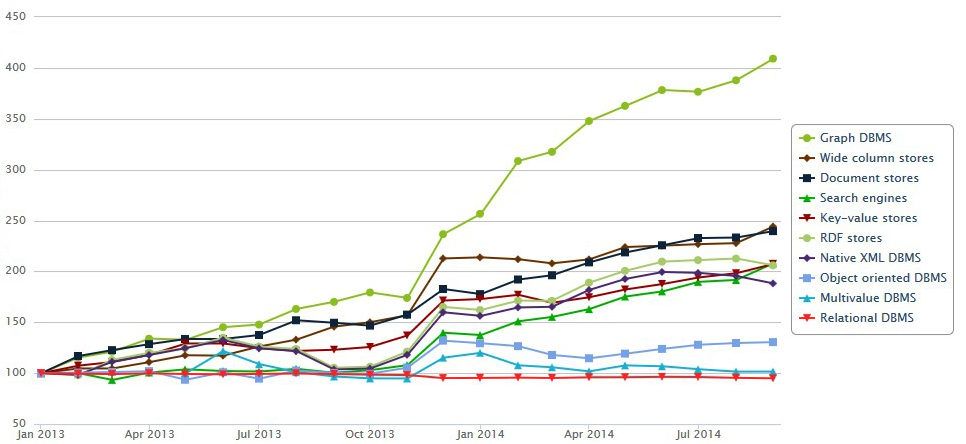
\includegraphics[width=\textwidth]{popgraph}
\caption{\textit{trend} di popolarità delle tecnologie NoSQL \cite{URL:dbengines}.}
\label{graphnosql}
\end{figure}

Sia i nodi sia le relazioni possono essere arricchite con delle proprietà e gli archi possono essere orientati o bidirezionali.

L’attrattiva di questa soluzione risiede nella semplicità con cui possono essere rappresentate le relazioni tra entità di una applicazione. Per questo motivo spesso sono impiegati 
in siti di \textit{e-commerce} per costruire un grafo di utenti e prodotti acquistati. Tramite questo grafo è possibile riuscire a predire con dei \textit{recommender system} \cite{recsys} quali nuovi prodotti 
un utente potrebbe essere interessato a comprare per fornire suggerimenti personalizzati.

I database a grafo possono essere interrogati per effettuare inferenze dirette o indirette sui dati memorizzati: verificare le relazioni tra i nodi, infatti, non richiede il 
completamento di costose operazioni di \textit{join}. Le analisi sui tipi di relazioni sono molto efficienti, a differenza degli altri tipi, molto meno ottimizzati. Aggiungere o rimuovere 
relazioni dal grafo risulta banale.

Prodotti attualmente impiegati in molti casi d’uso sono Neo4j, Titan e InfiniteGraph.

\begin{table}[ht]
\centering
\begin{tabular}{|l|l|}
\hline
\textit{Rank} & DBMS          \\ \hline
1             & Neo4j         \\
2             & Titan         \\
3             & OrientDB      \\
4             & Sparksee      \\
5             & Giraph        \\
6             & ArangoDB      \\
7             & InfiniteGraph \\
8             & Sqrrl         \\
9             & InfoGrid      \\
10            & FlockDB       \\ \hline
\end{tabular}
\caption{diffusione dei database a grafo, aggiornata a settembre 2014 \cite{URL:dbengines}.}
\end{table}

\chapter{Cloud computing}
\label{chap:cloud}

\section{Caratteristiche e modelli di servizi offerti}

Nel paragrafo \ref{par:crit} sono stati evidenziati i problemi che si devono solitamente affrontare durante la gestione di \textit{big data}, ovvero quelli riguardanti le modalità e l’ubicazione dei 
processi di elaborazione e memorizzazione. Nel capitolo \ref{chap:hadoop} è stato presentato Hadoop, un \textit{framework} progettato per elaborare grandi \textit{dataset} in modo distribuito, mentre nel 
\ref{chap:nosql} sono stati approfonditi i database NoSQL, tecnologie scalabili in grado di memorizzare e recuperare efficientemente molte informazioni. Questi due strumenti forniscono 
modalità adatte per la gestione di grandi moli di dati, ma ancora nessuna soluzione è stata proposta per risolvere il problema dell’ubicazione di questi processi. Nel corso di 
questo capitolo, pertanto, verranno analizzate le piattaforme di \textit{cloud computing}, degli strumenti per processare dati in remoto, che spesso si rivelano più adeguati dei \textit{client} locali.

Questi servizi si sono sviluppati soprattutto negli ultimi dieci anni, in risposta alle esigenze di molte imprese di decentralizzare la fase di elaborazione dei dati. A fronte del 
notevole aumento del volume di dati raccolti, infatti, numerose aziende hanno realizzato di possedere infrastrutture inadatte o troppo costose (spese di manutenzione, \textit{upgrade}, personale, 
energia elettrica, ecc.) per soddisfare le richieste dei propri sistemi. Diversi colossi informatici hanno ritenuto questa situazione una buona occasione per impiegare con maggiore 
produttività i loro \textit{data center} e per aggiungere una nuova cospicua fonte di guadagno al loro business. Sono nate così le piattaforme di \textit{cloud computing}, gruppi di servizi noleggiabili
da aziende o privati secondo dettagliate politiche di prezzi ed utilizzabili nella forma di \textit{web service}. Usufruendo delle potenti infrastrutture di aziende come Amazon, Google, IBM, 
Microsoft, ecc. le imprese ricevono la garanzia di elaborare e memorizzare le informazioni con grande velocità ed in modo sicuro (per via dei processi di criptografia e replicazione 
dei dati). 

Integrare questi servizi nelle applicazioni preesistenti risulta spesso semplice, per via delle API in diversi linguaggi di programmazione che vengono fornite agli sviluppatori. 
Beneficiando delle infrastrutture di queste imprese, i sistemi risultano scalabili e godono di disponibilità pressoché continua.  Le interfacce web, inoltre, rendono la gestione 
di questi servizi ancora più intuitiva.

Le piattaforme di \textit{cloud computing} differiscono per i servizi contenuti, le politiche dei prezzi ed altre caratteristiche minori, ma, generalmente, condividono i modelli di 
servizi offerti: \textit{Infrastructure as a Service} (IaaS), \textit{Platform as a Service} (PaaS) e \textit{Software as a Service} (SaaS).

Col modello IaaS il \textit{cloud provider} offre macchine fisiche o, più spesso, virtuali con \textit{hardware} configurabile oppure altre risorse, quali \textit{load balancer}, indirizzi IP, VLAN, 
\textit{client} per lo \textit{storage} di file, ecc. Queste risorse remote possono essere utilizzate per avviare macchine con sistema operativo personalizzato - tramite immagini di dischi 
preconfigurate - con cui eseguire qualunque tipo di computazione (ad esempio, è possibile utilizzarle per un \textit{cluster} di Hadoop). In questo modo gli utenti possono disporre 
di un numero di computer virtualmente illimitato con cui far fronte a qualunque tipo di esigenza. Collegandosi alle proprie macchine, spesso tramite il protocollo di rete SSH, 
è possibile infatti installare ed avviare su di esse dei propri programmi e raccogliere i risultati delle analisi effettuate nei \textit{data center} del \textit{cloud provider}.

Solitamente i costi di questi servizi sono proporzionali alla quantità di risorse utilizzate nel tempo e, pertanto, è consigliabile condurre analisi sull’effettiva economicità 
della soluzione. Per tale motivo spesso le macchine vengono avviate, impiegate per qualche elaborazione e subito spente, al fine di non pagare intervalli di inattività: questo 
approccio risulta praticabile per via dei ridotti tempi di accensione e spegnimento delle istanze remote.

Nel modello di PaaS i fornitori offrono delle risorse di elaborazione già configurate e pronte all’uso. Tipicamente vengono messe a disposizione macchine con un determinato 
sistema operativo e diversi \textit{software} preinstallati: ambienti d’esecuzione per linguaggi di programmazione (ad esempio la Java Virtual Machine), database, \textit{web server} e strumenti
di varia natura. Queste macchine possono essere utilizzate nel \textit{core} di un proprio sistema e, se adeguatamente selezionate, si rivelano molto adatte a sopportare grandi carichi 
di lavoro. Un servizio PaaS, ad esempio, potrebbe gestire le richieste fatte ad un sito web, ad una applicazione per smartphone, ad un servizio di telefonia, ecc.

Diversi \textit{provider}, come Google e Microsoft offrono anche delle funzionalità di \textit{load balancing}: all’aumentare delle richieste il \textit{provider} alloca dinamicamente nuove risorse per 
non far degradare il sistema nelle performance, senza che l’utilizzatore del servizio debba intervenire manualmente. I sistemi sono quindi capaci di scalare automaticamente e, 
pertanto, questi servizi di adattano bene ad ambienti \textit{real-time}.

Infine, col modello SaaS, i \textit{provider} noleggiano i propri \textit{software}, nascondendo agli utilizzatori i dettagli sulle infrastrutture sottostanti e sollevandoli dall’onere di configurare 
ed avviare delle macchine remote. Il modello SaaS viene talvolta definito come “\textit{software on-demand}”, proprio perché gli utenti possono fare uso delle applicazioni offerte nella 
piattaforma in relazione alle loro esigenze. È compito del \textit{cloud provider} assicurarsi che i prodotti siano sempre disponibili e funzionanti, bilanciando i carichi di lavoro e 
manutenendo ed evolvendo il \textit{software} (i cambiamenti sono trasparenti agli utenti).

Il modello SaaS permette agli investitori di utilizzare soluzioni già in commercio e risparmiare denaro evitando l’acquisto di \textit{hardware} ed i costi di manutenzione: in questo 
modo è possibile orientarsi verso altri obiettivi.

Tutti i modelli, tuttavia, presentano lo svantaggio di dover memorizzare i dati degli utenti nei \textit{client} del \textit{cloud provider}, esponendoli al rischio di accessi non autorizzati. 
Per ovviare a questi problemi i fornitori dei servizi solitamente offrono diverse garanzie (i file vengono divisi in più parti, criptati e sparsi in \textit{data center} diversi), ma 
gli utenti possono anche usufruire di servizi di criptazione di terze parti per assicurarsi maggiore protezione.

La piattaforma per l’analisi di \textit{big data} sviluppata per questo studio necessitava di servizi di \textit{cloud computing} per potere adoperare \textit{framework} come Hadoop e per beneficiare 
della scalabilità garantita dal \textit{cloud provider}. Per tale motivo essa presenta una architettura ibrida, con diverse componenti \textit{cloud}. È stato comunque 
dimostrato \cite{accenture:cloud} che le soluzioni \textit{cloud} costituiscono, dal punto di vista economico, 
una valida alternativa a quelle \textit{bare-metal} per molti casi d’uso e sono pertanto suggerite anche in assenza di necessità simili a quelle di questo caso di studio.

La Google Cloud Platform è stata preferita alle altre piattaforme per la varietà di tecnologie nel suo portfolio, per la superiorità nelle prestazioni rispetto ai 
concorrenti \cite{URL:gcpbest1} \cite{URL:gcpbest2}, per la sua semplicità di utilizzo, per la molteplicità di strumenti offerti agli sviluppatori 
(\textit{plugin} per IDE, \textit{script} di configurazione e \textit{deploy}, ecc.) e per la sua effettiva economicità (per provare i servizi ed eseguire tutti gli esperimenti della piattaforma 
sono stati consumati in totale circa 12\$).


\section{Google Cloud Platform}
\label{chap:gcp}

La Google Cloud Platform (GCP) è una raccolta di alcune delle tecnologie sviluppate da Google ed attualmente utilizzate internamente dall’azienda per garantire il corretto 
funzionamento dei suoi prodotti, quali Gmail, YouTube, il motore di ricerca ed altri.

La piattaforma è stata resa disponibile al pubblico a partire dal 2008 con l’obiettivo di noleggiare ad aziende e privati gli stessi strumenti adoperati da Google nella forma 
di \textit{web service}. Con essa Google è entrata nel panorama dei \textit{cloud provider}, in diretta competizione con Amazon Web Services (AWS), Azure di Microsoft, SoftLayer e BlueMix di IBM, ecc.

Nel corso degli anni la piattaforma di Google è stata evoluta, migliorando i suoi prodotti, introducendo nuovi servizi, fornendo ulteriori API agli sviluppatori ed aggiornando 
le politiche dei prezzi, conformemente ai competitori.

Secondo le modalità tipiche dei servizi di \textit{cloud computing}, gli interessati alle tecnologie offerte nel portfolio possono utilizzare i prodotti di cui hanno bisogno dietro un 
opportuno compenso. Noleggiando le proprie infrastrutture ed i propri \textit{software}, pertanto, Google si assicura una cospicua fonte di guadagno (come anticipato nel paragrafo \ref{par:money}) 
e permette agli sviluppatori di adoperare potenti strumenti, adatti ad elaborare efficientemente \textit{big data}.

I servizi inclusi nella piattaforma sono di natura eterogenea e rientrano nei modelli di IaaS, PaaS e SaaS. Tutti beneficiano di diverse qualità come scalabilità e disponibilità, 
assicurano protezione e replicazione dei dati trattati e garantiscono elevate performance, indipendentemente dal numero di richieste cui devono rispondere. Le tecnologie offerte 
dalla Google Cloud Platform sono, in generale, orientate all’elaborazione o alla memorizzazione delle informazioni; talvolta costituiscono servizi specifici per le applicazioni. 
Di seguito viene presentato un elenco di alcuni dei prodotti principali inclusi nella piattaforma:

Compute Engine: IaaS che permette la creazione di una o più macchine virtuali con \textit{hardware} configurabile dall’utente. Può essere utilizzata per creare \textit{cluster} di computer, che 
saranno collegati tra loro attraverso la fibra ottica privata di Google;

App Engine: PaaS utilizzata per sviluppare ed ospitare applicazioni nei \textit{data center} di Google. L’SDK supporta diversi linguaggi di programmazione ed è compatibile con i 
maggiori \textit{framework}. Google si occupa di gestire le richieste fatte alle applicazioni utilizzanti App Engine, amministrare i database e bilanciare i carichi di lavoro;

Cloud SQL: database relazionale MySQL che gestisce, in modo trasparente all’utente, la replicazione ed il \textit{backup} dei dati, l’aggiornamento del sistema ed il recupero automatico 
in caso di errori. È capace di processare efficientemente miliardi di tuple e può essere usato dai tradizionali strumenti di gestione di database relazionali;

Cloud Storage: servizio per la memorizzazione di dati, simile ai tradizionali servizi di \textit{file hosting};

Cloud Datastore: database NoSQL \textit{schema-less}, ideale per memorizzare dati non strutturati. Supporta transazioni ACID e \textit{query SQL-like}. Google provvede allo \textit{sharding} ed alla 
replicazione dei dati;

Big Query: IaaS che permette di analizzare grandi \textit{dataset} in pochi secondi eseguendo \textit{query SQL-like}, ideale come strumento per acquisire in tempo reale comprensione su \textit{big data}.

Tra i prodotti presentati alcuni sono stati utilizzati per la piattaforma oggetto di questo lavoro e saranno, pertanto, presentati nel dettaglio.


\subsection{Google Compute Engine}
\label{par:GCE}

Google Compute Engine (GCE) è uno dei servizi principali della GCP che permette agli utenti di avviare e controllare remotamente macchine virtuali (VM) in esecuzione nei 
\textit{data center} di Google.

Gli utenti hanno la possibilità di configurare le macchine che saranno avviate e, una volta attive, utilizzare queste istanze per effettuare qualsiasi tipo di operazione. 
Nello specifico, essi devono specificare il sistema operativo ed il tipo di macchina. GCE è compatibile con molti sistemi operativi e distribuzioni, alcuni gratuiti, altri 
a pagamento. Alcuni tra quelli nativamente supportati sono Debian, CentOS, openSUSE, Red Hat, FreeBSD e Windows Server, ma viene anche offerta la possibilità di caricare 
immagini personalizzate, che meglio rispondono alle esigenze degli utilizzatori. Il tipo di macchina, invece, determina le specifiche fisiche della VM, come il quantitativo 
di memoria disponibile o il numero di \textit{core} virtuali. Il tipo deve essere scelto tra quelli offerti da Google, che, per comodità, raggruppa l’offerta in quattro categorie di
macchine: \textit{standard}, \textit{high CPU}, \textit{high memory}, \textit{small}. Gli utenti possono pertanto scegliere, in relazione all’utilizzo che sarà fatto delle istanze, se avviare macchine con molta 
memoria o preferire una maggiore potenza di elaborazione oppure propendere per soluzioni economiche e con poche risorse. La tabella \ref{table:GCE} riassume l’attuale proposta di Google 
e descrive i tipi di VM.

\begin{table}[ht]
\centering
\begin{tabular}{|l|l|l|l|}
\hline
Tipo macchina  & # CPU & Memoria (GB) & Prezzo (\$/h) \\ \hline
n1-standard-1  & 1        & 3,75         & 0,077       \\
n1-standard-2  & 2        & 7,50         & 0,154       \\
n1-standard-4  & 4        & 15           & 0,308       \\
n1-standard-8  & 8        & 30           & 0,616       \\
n1-standard-16 & 16       & 60           & 1,232       \\
n1-highmem-2   & 2        & 13           & 0,18        \\
n1-highmem-4   & 4        & 26           & 0,36        \\
n1-highmem-8   & 8        & 52           & 0,72        \\
n1-highmem-16  & 16       & 104          & 1,44        \\
n1-highcpu-2   & 2        & 1,80         & 0,096       \\
n1-highcpu-4   & 4        & 3,60         & 0,192       \\
n1-highcpu-8   & 8        & 7,20         & 0,384       \\
n1-highcpu-16  & 16       & 14,40        & 0,768       \\ \hline
\end{tabular}
\caption{offerta di Compute Engine. Una CPU virtuale è implementata come un singolo \textit{hyperthread} su un processore Intel Sandy Bridge Xeon o Intel Ivy Bridge Xeon a 2.6GHz 
(due CPU virtuali corrispondono ad un intero \textit{core} fisico). I prezzi sono relativi all'Europa.}
\label{table:GCE}
\end{table}

Quando vengono spente dall’utente, le istanze di GCE sono distrutte e le risorse a loro dedicate vengono riutilizzate per nuove VM; con questo processo tutti i dati memorizzati
sul disco dall’utente vengono perduti. Per risolvere questo problema, Google offre la possibilità di utilizzare dischi persistenti, risorse assimilabili agli \textit{hard drive} 
comunemente collegati ai personal computer. Essi si presentano come la soluzione primaria per la memorizzazione di dati in modo persistente. Un disco può essere collegato 
e scollegato ad una VM secondo le preferenze dell’utente e può essere programmato per distruggersi o rimanere in funzione quando l’istanza cui è collegato viene spenta. Nel 
secondo caso i dati memorizzati al suo interno non vengono persi e l’utente può collegare il disco ad una nuova istanza. In fase di configurazione di un disco l’utente può 
scegliere se creare un disco \textit{standard} oppure un SSD: come per i tipi di macchina, anche i dischi hanno performance e prezzi differenti.

Le macchine virtuali possono essere utilizzate indipendentemente oppure possono essere collegate tra loro per formare un \textit{cluster}. Google mette a disposizione, ad esempio, 
degli \textit{script} per effettuare il \textit{deploy} di un \textit{cluster} Hadoop avente caratteristiche impostate dall’utente (numero e tipologia di nodi, file da copiare sulle macchine all’avvio, 
\textit{file system}, ecc.). Le macchine sono collegate tra loro attraverso la fibra ottica di Google e, pertanto, le connessioni registrano basse latenze: il trasferimento di dati 
tra i nodi del \textit{cluster} risulta molto veloce e GCE rappresenta una buona infrastruttura per il calcolo distribuito.

Tutte le istanze sono collegate ad Internet e posso essere collegate in una rete interna, eventualmente protetta con un \textit{firewall}. Ciascuna di esse, inoltre, possiede un 
proprio indirizzo IP e può essere identificata tramite una risoluzione DNS. 

Le risorse di GCE possono essere facilmente gestite attraverso lo strumento da riga di comando o tramite la \textit{web console} degli sviluppatori della piattaforma (in entrambi
i casi il protocollo SSH viene utilizzato per collegarsi alle istanze remote). I \textit{software} possono poi interagire con le macchine utilizzando le RESTful API per diversi 
linguaggi offerte agli sviluppatori (Java, Python, Ruby, .NET, Go, PHP, Objective C, ecc.). Esse solitamente utilizzano OAuth 2.0 per completare l’autenticazione e per integrare
GCE con altri prodotti della piattaforma come Cloud Storage.

Google non garantisce, ad ogni modo, che le istanze siano in esecuzione per il 100\% del tempo, pertanto è compito degli utenti assicurarsi che il proprio servizio possa 
ripristinare il proprio stato a seguito di un guasto imprevisto; diversi accorgimenti vengono comunque suggeriti per progettare sistemi robusti.

\subsection{Google Cloud Storage}

Google Cloud Storage (GCS) rappresenta una delle tre soluzioni offerte nella piattaforma per la memorizzazione dei dati, insieme a Cloud SQL e Cloud Datastore. Mentre questi ultimi
due prodotti costituiscono dei veri e propri database, GCS è un più semplice servizio di file \textit{storage} nel \textit{cloud}. Con esso gli utenti possono arrivare a memorizzare diversi terabyte 
di dati, pagando in relazione all’ammontare di dati trasferiti ed allo spazio fisico occupato (il prezzo è di circa 0.026\$/GB/mese). I dati possono essere memorizzati in uno 
o più \textit{data center} di Google (Stati Uniti, Unione Europea ed Asia), che garantisce agli utilizzatori elevate velocità di lettura, continua disponibilità e, soprattutto, scalabilità.
Il servizio risulta, pertanto, anche adatto a distribuire in \textit{download} diretto file molto grandi o molto richiesti.

GCS è una tecnologia di \textit{storage} rivolta agli sviluppatori, poiché i file memorizzati possono essere utilizzati da altri prodotti della piattaforma di Google. Per questo motivo 
viene spesso utilizzato insieme ad altri servizi, ad esempio Compute Engine, App Engine e Big Query. Gli utenti che non sono interessati a sviluppare \textit{software} possono, invece, 
utilizzare il più noto Google Drive, un più semplice servizio di \textit{hosting}. Ad ogni modo, utilizzando il Google Drive SDK, è possibile integrare i due servizi, per offrire agli 
utenti finali i file caricati su Cloud Storage.

In GCS tutti i dati vengono contenuti in un progetto, che consiste di un insieme di utenti abilitati a gestire i file, un insieme di API attivate ed impostazioni di fatturazione 
ed autenticazione. Ogni utente può gestire uno o più progetti e può creare, all’interno di un progetto, un numero arbitrario di \textit{bucket}. Essi rappresentano i contenitori dei file
e sono assimilabili a delle cartelle: tutti gli oggetti caricati in GCS devono essere inseriti in un \textit{bucket}. A differenze delle cartelle, però, i \textit{bucket} non possono essere annidati
e non possono essere condivisi tra più progetti. Ogni \textit{bucket} è caratterizzato da un identificativo univoco e permette di configurare i privilegi da assegnare agli utenti che 
vogliono accedervi. Gli oggetti di GCS non possono essere condivisi tra più \textit{bucket} e possiedono due componenti: dati e metadati. I dati rappresentano il file da memorizzare, 
mentre i metadati sono delle coppie chiave-valore che descrivono delle qualità dell’oggetto.

GCS offre una forte \textit{read-after-write consistency} per tutte le operazioni di \textit{upload} e cancellazione. Questo significa che un oggetto appena caricato può subito essere scaricato, 
rimosso o ispezionato nei suoi metadati. Allo stesso modo risulta impossibile accedere ad un oggetto che è stato appena cancellato. Dal punto di vista della disponibilità, le 
operazioni su GCS sono atomiche: gli oggetti caricati sono accessibili solo se perfettamente integri. I file corrotti o parziali non possono essere letti, così come quelli ancora 
in fase di \textit{upload}.

Come per Compute Engine, anche le risorse di Cloud Storage possono essere gestite in diversi modi: interfaccia da riga di comando, \textit{web console} ed API (XML, JSON, ecc.). I \textit{software} 
possono interagire con il servizio attraverso una delle librerie offerte da Google, disponibili per tanti linguaggi di programmazione. Anche GCS utilizza OAuth 2.0 per gestire i
meccanismi di autenticazione e autorizzazione.

\chapter{Piattaforma cloud per l'analisi di big data}
\label{chap:platform}

\section{Contesto del lavoro}

Le tecnologie presentate nei precedenti capitoli sono state impiegate per lo sviluppo di una piattaforma \textit{cloud} per l’analisi di \textit{big data} provenienti da \textit{social network}, i cui 
componenti saranno illustrati nel corso di questo capitolo.

L’origine di tale strumento risiede nell’esigenza avvertita da Vox, Osservatorio Italiano sui Diritti, di monitorare le zone italiane dove omofobia, razzismo, discriminazione verso
i disabili, misoginia ed antisemitismo sono maggiormente diffusi. L’ambizioso obiettivo del progetto, infatti, è lo sviluppo di una Mappa dell’Intolleranza, un mezzo capace di 
evidenziare i luoghi affetti da questi gravi problemi di discriminazione, attraverso l’analisi di \textit{tweet} in lingua italiana geolocalizzati. 

L’idea di questo strumento non è nuova: gli studenti della Humboldt State University in California hanno sviluppato nel 2013 la Hate Map (in figura \ref{humbimg}), una mappa di calore interattiva 
in grado di mostrare le principali zone degli Stati Uniti da cui provenivano \textit{tweet} razzisti, omofobi e contro le persone diversamente abili. Il loro lavoro ha consentito importanti 
osservazioni di carattere sociale: è stato riscontrato, ad esempio, che la maggior parte dei messaggi d’odio avevano origine in piccole città o aree rurali piuttosto che in grandi 
metropoli.

\begin{figure}[ht]
\centering
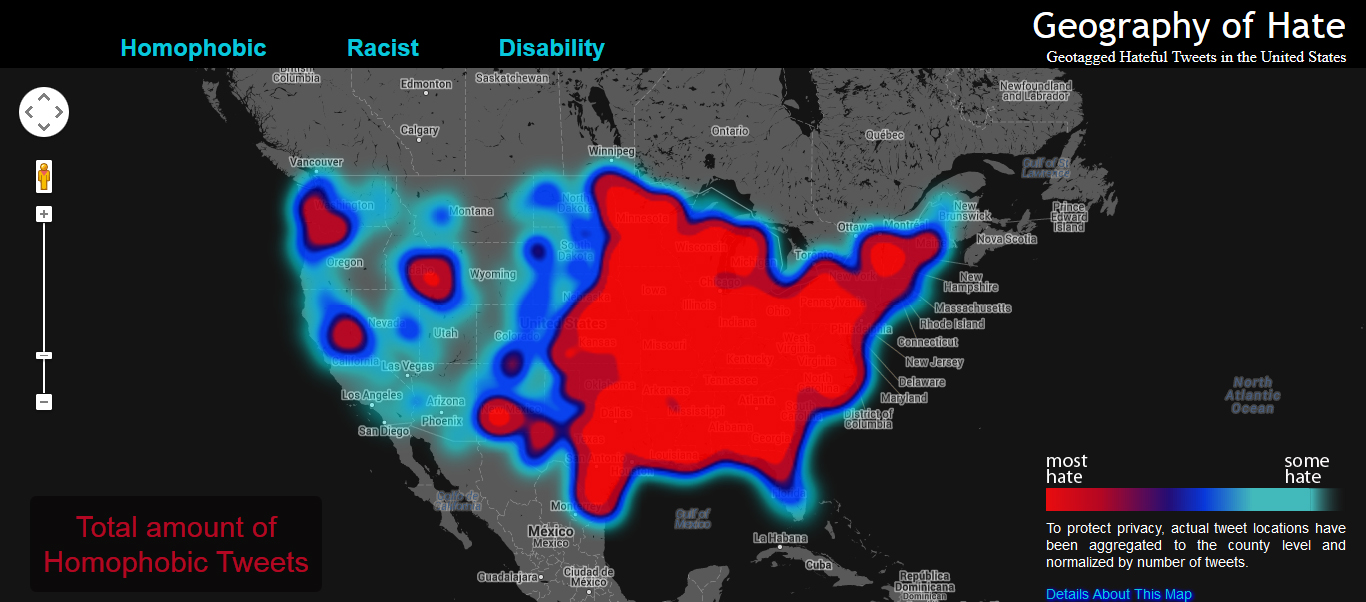
\includegraphics[width=\textwidth]{hatemaphum}
\caption{Hate Map degli Stati Uniti d'America\protect\footnotemark.}
\label{humbimg}
\end{figure}

La Mappa dell’Intolleranza di Vox è pensata per offrire alle amministrazioni locali italiane uno strumento per scoprire le aree più a rischio, al fine di agire concretamente sul 
territorio per risolvere i problemi di discriminazione. Recenti statistiche dimostrano quanto importante sia operare attivamente in tale direzione: solo nel 2013, il 25\% degli 
omosessuali è stato vittima di violenza, 6743000 donne hanno subito abusi fisici o sessuali ed il 45\% dei giovani si è dichiarato xenofobo o diffidente degli stranieri \cite{URL:vox}.

Il ruolo dei \textit{social network} in questo contesto è essenziale, poiché essi permettono di veicolare ed alimentare sentimenti di odio verso il prossimo con grande facilità. Uno studio 
sistematico dei messaggi discriminatori pubblicati dagli utenti potrebbe, però, permettere di prevenire l’insorgere di episodi violenti e situazioni spiacevoli.

\footnotetext{\url{http://users.humboldt.edu/mstephens/hate/hate_map.html}}

Il progetto avviato da Vox risulta essere tanto importante, quanto complesso. Fa emergere, infatti, diverse problematiche di natura linguistica e tecnologica alle quali diverse 
facoltà italiane stanno facendo fronte collaborando, al fine di produrre uno strumento affidabile e preciso.

La piattaforma che sarà ora descritta permette un importante passo avanti nella realizzazione del progetto della Mappa dell’Intolleranza, poiché si prefigge di essere 
l’infrastruttura portante del sistema ed uno strumento scalabile per la raccolta e l’analisi di grandi moli di dati.


\section{Architettura della piattaforma}

Nello sviluppo della piattaforma è stato seguito un approccio modulare, in linea con le \textit{best practice} dell’ingegneria del \textit{software}. Questa scelta progettuale ha portato allo 
sviluppo di un sistema dotato di moduli indipendenti tra loro, facilmente manutenibili e concepiti per portare a termine determinati compiti in modo autonomo. Il \textit{software} 
beneficia, nel complesso, di diverse importanti qualità, tra cui spiccano \textbf{evolvibilità} e \textbf{scalabilità}. La prima risulta essenziale per una piattaforma costituente l’infrastruttura 
di un sistema complesso, che, verosimilmente, cambierà nel corso del tempo per rispondere a nuove esigenze. Nel suo \textit{core}, infatti, la piattaforma è predisposta ad accettare nuovi 
moduli, con cui potrà effettuare operazioni attualmente non supportate, anche molto differenti tra loro. Il requisito di scalabilità, d’altronde, è imprescindibile per un \textit{software}
finalizzato alla gesione di \textit{big data}, nonostante la dimensione dei \textit{tweet} finora raccolti permettesse l’utilizzo di tecnologie tradizionali per lo \textit{storage} ed il processing. In fase di sviluppo, invece, 
si è supposto di dover elaborare più informazioni di quelle possedute e sono stati presi tutti gli accorgimenti del caso, impiegando tecnologie ed algoritmi adatti per i \textit{big data}. 
Il sistema è stato pertanto contestualizzato in una situazione futura, simulando lunghi periodi di attività e ipotizzando di aver raccolto molti più dati di quelli attualmente a 
disposizione.

Combinando i moduli che costituiscono il sistema è possibile eseguire delle attività più complesse, dette \textbf{\textit{task}}. Nella versione iniziale della piattaforma l’attenzione è stata posta 
sui \textit{task} orientati alla raccolta e all’elaborazione di informazioni, tralasciando i \textit{task} di \textit{data visualization}. Tra i \textit{task} implementati, particolare attenzione è stata posta su quelli 
destinati a trattare in modo diretto grandi moli di dati, detti \textit{big data critic}. Questi \textit{task} hanno richiesto, infatti, l’utilizzo di tecnologie ed algoritmi scalabili e le loro 
performance sono state oggetto dello studio riportato nel capitolo \ref{chap:esp}.

Il \textit{software} è stato sviluppato in Java, lo stesso linguaggio utilizzato dalle librerie che esso utilizza come dipendenze. Le tecnologie specifiche per i \textit{big data} impiegate, inoltre, 
espongono API in questo linguaggio, lasciando, di fatto, poco margine di scelta in fase realizzativa. A fronte del gran numero di \textit{software} di terze parti e librerie necessari 
per completare i \textit{task} della piattaforma, è stato utilizzato il \textit{framework} Maven per gestire in modo agevole le dipendenze e rendere il programma facilmente evolvibile.


\section{Obiettivi del lavoro di analisi}
\label{par:method}

La piattaforma realizzata, nonostante sia impiegabile in diversi modi, è stata utilizzata per eseguire due esperimenti specifici, che hanno indirizzato lo sviluppo verso 
determinati moduli piuttosto che altri.

Il primo obiettivo del lavoro è stato scoprire se l'utilizzo di tecnologie per il calcolo distribuito si rivela una soluzione efficace per risolvere i problemi di elaborazione di \textit{big data}.
Per ottenere dei risultati significativi, a diversi \textit{cluster} sono stati fatti eseguire sia \textit{task} \textit{data intensive}, sia \textit{task} su piccoli \textit{dataset}. 
Sono stati misurati sia i tempi di avvio che quelli di spegnimento dei \textit{cluster} ed è stato effettuato un confronto con le prestazioni ottenute da macchine tradizionali.

Il secondo obiettivo, invece, è stato quello di individuare delle caratteristiche linguistiche salienti tra i dati raccolti, 
analizzandoli dal punto di vista statistico. Ignorando la semantica dei \textit{tweet} si è ipotizzato di riuscire comunque a trovare delle peculiarità tra i messaggi 
di odio indirizzati a determinate categorie di persone. Tali caratteristiche potrebbero essere utilizzate, ad esempio, per scoprire nuovi messaggi, ignorati
nelle precedenti sessioni di campionamento.

Per eseguire gli esperimenti, nella fase iniziale del lavoro, è stato raccolto da Twitter un numero significativo di messaggi, che sono stati raggruppati in base alla loro tipologia
di intolleranza (contro le donne, contro i disabili, contro gli omosessuali, ecc.). Le categorie più ricche di messaggi sono state indicizzate durante il primo esperimento. Dai risultati ottenuti, 
durante il secondo esperimento, sono state calcolate delle distribuzione di probabilità dei termini utilizzati nei \textit{tweet}.
Tali distribuzioni saranno più informative all’aumentare dei messaggi raccolti, pertanto i risultati ottenuti potrebbero migliorare a seguito di sessioni più lunghe di raccolta di dati.

Per far emergere dai \textit{tweet} le parole più caratteristiche si è reso necessario confrontare le distribuzioni di probabilità con una di riferimento che approssimasse quanto 
meglio possibile dei testi generici in lingua italiana. Infatti, i termini frequenti nei \textit{tweet} e non d’uso comune nella lingua scritta appartengono all’insieme di parole più 
peculiari per la categoria in esame e sono di interesse per lo studio. Ad esempio, il termine ``\textit{giorno}'' è molto impiegato sia nei testi in italiano, sia nei \textit{tweet} di odio contro le donne
e quindi non può essere utile per individuare comportamenti misogini. Al contrario, il termine ``\textit{inchiavabile}'' - mi venga perdonato l'utilizzo dell'aggettivo dispregiativo - 
è usato con ricorrenza solo nei \textit{tweet} e può essere d'aiuto ad identificare messaggi contro le donne. Una distribuzione che approssimasse bene la nostra lingua è 
stata ottenuta indicizzando itWaC, una ricca raccolta di testi in italiano (per dettagli sul corpus
si rimanda al paragrafo \ref{esphadoop:dataset}). I termini più significativi per i \textit{tweet} discriminatori sono stati individuati calcolando la divergenza di Kullback-Leibler 
tra la distribuzione di probabilità dei messaggi e quella di itWaC (ulteriori dettagli sono forniti nei paragrafi \ref{par:KLD} e \ref{esptweet:proto}). Ordinando i termini per 
significatività descrescente nei \textit{tweet} è stato possibile evidenziare nelle prime posizioni i contenuti più peculiari per ogni gruppo.

Di seguito vengono analizzati i componenti della piattaforma che sono stati sviluppati per portare a termine il lavoro.


\section{Crawler}

Uno dei moduli più importanti della piattaforma è il \textit{crawler}. Esso permette di raccogliere dati da una generica sorgente informativa per effettuare delle elaborazioni in tempo reale 
o in un momento successivo.

Il sistema può eseguire diversi tipi di \textit{crawler}. Uno specifico per Twitter è stato già implementato e costituisce un componente essenziale per il progetto della ``\textit{Mappa dell’Intolleranza}''. 
Esso fa utilizzo della \textbf{Streaming API} di Twitter per ricevere i \textit{tweet} provenienti dal flusso globale di messaggi che soddisfano dei criteri fissati dallo sviluppatore. Twitter offre 
diversi \textit{streaming endpoint}, ciascuno adatto per particolari casi d’uso. L’\textit{endpoint} scelto per questo \textit{crawler} è quello pubblico, adatto quando si vogliono raccogliere dati 
di pubblico dominio su utenti od argomenti specifici, poiché è in grado di filtrare automaticamente i messaggi di interesse per il \textit{client} tra quelli presenti nel flusso di \textit{tweet}. 
Gli altri \textit{endpoint} sono quello specifico per gli utenti, che raccoglie tutti i dati (anche quelli privati) riguardanti un determinato utente (utilizzato, ad esempio, per i \textit{client} 
mobili per Twitter di terze parti) e quello per i siti (la versione multi-utente del precedente).

Per ricevere informazioni da Twitter, il \textit{client} deve autenticarsi come sviluppatore ed effettuare una richiesta al \textit{social network} tramite l’API, specificando i contenuti che è 
interessato a ricevere. Pervenuta la richiesta, Twitter apre una connessione HTTP permanente con il \textit{client} e gli invia dati in tempo reale, nella forma di documenti JSON, attraverso
questo canale. È compito del \textit{client} leggere in modo progressivo le informazioni che riceve da questa sorgente informativa e restare in ascolto di nuovi dati. Questo meccanismo di
interazione si contrappone a quello dalla REST API, con cui il \textit{client} può chiedere una particolare informazione al \textit{social network} tramite un’interrogazione che utilizza una connessione
temporanea per veicolare il dato. La natura della Streaming API, pertanto, richiede una particolare attenzione in fase di sviluppo del \textit{client}, che dovrà esser capace di consumare 
dati in tempo reale, senza causare \textit{bottleneck}. Per convertire velocemente i documenti JSON ricevuti con l’API in oggetti Java è stato perciò impiegato Jackson, un \textit{JSON-processor} 
capace di estrarre dai documenti degli attributi specificati dall’utente (corpo del messaggio, autore, identificativo, provenienza, ecc.) ed ignorare tutti gli altri. 

Il \textit{crawler} per Twitter è stato progettato per raccogliere messaggi in una determinata lingua contenti specifiche \textit{keyword}. Per realizzare la ``\textit{Mappa dell’Intolleranza}'' si rende necessario 
possedere \textit{tweet} potenzialmente omofobi, razzisti, discriminanti verso disabili, misogini ed antisemiti. Per comodità questi messaggi sono stati suddivisi in classi numerate 
progressivamente (1: omofobia, 2: razzismo, 3: disabilità, 4: misoginia, 5: antisemitismo). Per raccogliere questi \textit{tweet}, un gruppo di psicologi della Università degli Studi di Roma 
"La Sapienza" ha fornito, per ogni classe, un insieme di termini, detti \textit{seed}, utilizzati con accezione spesso discriminatoria in contesti quotidiani. Un lavoro successivo, inoltre, 
ha permesso di ampliare questo lessico tramite l’uso di sinonimi, variazioni morfologiche (nel genere e nel numero) e risorse esterne, quali BabelNet e Morph-it!. 
Tutti i \textit{seed} raccolti sono stati utilizzati per raccogliere i \textit{tweet} appartenenti a ciascuna classe.

\begin{table}[ht]
\centering
\begin{tabular}{|l|l|l|l|}
\hline
frocio       & kecca      & bocchinari  & rottinculo    \\ \hline
froci        & checche    & bokkinari   & passiva       \\ \hline
frocie       & kekke      & deviato     & passivo       \\ \hline
froce        & invertito  & deviati     & passive       \\ \hline
ricchione    & invertite  & deviate     & passivi       \\ \hline
rikkione     & inverite   & deviate     & leccafica     \\ \hline
ricchionazzo & invertiti  & camionista  & leccafiche    \\ \hline
rikkionazzo  & pervertito & camioniste  & culanda       \\ \hline
ricchioni    & pervertita & marchettaro & travestito    \\ \hline
rikkioni     & pervertiti & marchettari & travestiti    \\ \hline
finocchio    & pervertite & sodomita    & travone       \\ \hline
finokkio     & pompinaro  & sodomiti    & travoni       \\ \hline
finocchi     & pompinari  & culattone   & ciuccia cazzi \\ \hline
finokki      & bocchinaro & culattoni   & ciuccia cazzo \\ \hline
checca       & bokkinaro  & piglianculo & succhia cazzo \\ \hline
culo rotto   & culi rotti & & \\ \hline
\end{tabular}
\caption{\textit{seed} classe 1.}
\end{table}

\begin{table}[ht]
\centering
\begin{tabular}{|l|l|l|l|}
\hline
negro    & terrone         & beduino           & zingare         \\ \hline
negri    & bangla          & beduini           & muso giallo     \\ \hline
negra    & rumeno di merda & polentone         & musi gialli     \\ \hline
negre    & rumena di merda & polentoni         & muso da scimmia \\ \hline
negretto & rumeni di merda & polentona         & musi da scimmia \\ \hline
negretta & rumene di merda & polentone         & kebabbaro       \\ \hline
negretti & romeno di merda & albanese di merda & kebabbari       \\ \hline
negrette & romeni di merda & albanesi di merda & kebabbara       \\ \hline
terrone  & romena di merda & zingaro           & kebabbare       \\ \hline
terroni  & romene di merda & zingari           & crucco          \\ \hline
terrona  & mangiarane      & zingara           & crucchi         \\ \hline
\end{tabular}
\caption{\textit{seed} classe 2.}
\end{table}

\begin{table}[ht]
\centering
\begin{tabular}{|l|l|l|l|}
\hline
handicappato & storpia     & nana      & quattrocchi    \\ \hline
handicappati & storpie     & nane      & cecato         \\ \hline
handicappata & mongoloide  & spastico  & cecati         \\ \hline
handicappate & mongoloidi  & spastici  & cecata         \\ \hline
andicappato  & cerebroleso & spastica  & cecate         \\ \hline
andicappati  & cerebrolesi & spastiche & mongoflettico  \\ \hline
andicappata  & cerebrolesa & zoppo     & mongoflettici  \\ \hline
andicappate  & cerebrolese & zoppi     & mongoflettica  \\ \hline
storpio      & nano        & zoppa     & mongoflettiche \\ \hline
storpi       & nani        & zoppe     &                \\ \hline
\end{tabular}
\caption{\textit{seed} classe 3.}
\end{table}

\begin{table}[ht]
\centering
\begin{tabular}{|l|l|l|l|}
\hline
troia      & scrofe        & zoccoletta   & sfasciolacazzi \\ \hline
troie      & sgualdrina    & zoccolette   & culona         \\ \hline
troietta   & sgualdrine    & mignotta     & culone         \\ \hline
troiette   & sciacquetta   & mignotte     & frigida        \\ \hline
troiona    & sciacquette   & mignottone   & frigide        \\ \hline
troione    & peripatetica  & bocchinara   & figa di legno  \\ \hline
puttana    & peripatetiche & bocchinare   & fighe di legno \\ \hline
puttane    & meretrice     & pompinara    & battona        \\ \hline
puttanella & meretrici     & pompinare    & battone        \\ \hline
puttanelle & cicciona      & cagna        & ciuccia cazzi  \\ \hline
bagascia   & ciccione      & cagne        & cesso          \\ \hline
bagasce    & vacca         & strappona    & cessa          \\ \hline
baldracca  & vacche        & strappone    & cesse          \\ \hline
baldracche & zoccola       & smandrappona & sfigata        \\ \hline
scrofa     & zoccole       & smandrappone & sfigate        \\ \hline
\end{tabular}
\caption{\textit{seed} classe 4.}
\end{table}

\begin{table}[ht]
\centering
\begin{tabular}{|l|l|}
\hline
ebreo ai forni & ebree di merda \\ \hline
ebrei ai forni & rabbino        \\ \hline
ebrea ai forni & rabbini        \\ \hline
ebree ai forni & giudeo         \\ \hline
ebreo di merda & giudea         \\ \hline
ebrei di merda & giudei         \\ \hline
ebrea di merda &                \\ \hline
\end{tabular}
\caption{\textit{seed} classe 5.}
\end{table}

Per un corretto funzionamento del \textit{crawler} è richiesto un file di configurazione apposito. Al suo interno l’utente deve specificare alcuni parametri: le credenziali da sviluppatore 
di Twitter, la lingua dei messaggi che è interessato a raccogliere (per il caso di studio è stata scelta quella italiana), le classi di interesse (coi rispettivi \textit{seed}) ed la durata 
delle sessione di \textit{crawling} per ciascuna classe. Nel file di configurazione, inoltre, l’utente può specificare dei filtri da applicare ai \textit{tweet} in arrivo e degli \textit{handler} per gestire 
i \textit{tweet} che hanno superato questi controlli.

I filtri sono stati implementati per dare la possibilità all’utente di bloccare determinati messaggi in base a delle loro caratteristiche (contenuto, provenienza, autore, ecc.) e 
dotare il modulo di un meccanismo di protezione dallo spam. Effettuando lunghe sessioni di \textit{crawling} è emerso, infatti, che diversi \textit{spam bot} impiegavano alcuni dei \textit{seed} delle classi
per promuovere siti web di carattere pornografico (cosa consentita dai termini di utilizzo di Twitter) o per campagne pubblicitarie di varia natura, producendo messaggi inutili per
il caso di studio. Mediante i filtri sviluppati questi ed altri messaggi sono stati bloccati, al fine di non alterare le distribuzioni di probabilità dei termini delle classi ed i 
risultati stessi delle analisi. L’utente è libero di non impiegare nessun filtro, utilizzarne alcuni già implementati o scriverne di nuovi.

Gli \textit{handler}, invece, sono i moduli preposti alla gestione dei \textit{tweet} che hanno superato i controlli dei filtri che sono stati attivati. Anche in questo caso l’utente può aggiungere
delle classi al sistema per eseguire nuove operazioni, oppure impiegare una già presente nella piattaforma. Gli \textit{handler} possono eseguire azioni di qualsiasi natura: memorizzare le 
informazioni inerenti un \textit{tweet} in un database (locale o in \textit{cloud}), condurre analisi di vario genere, serializzare il contenuto dei messaggi in un file di testo, ecc. Quest’ultima 
operazione era quella necessaria al caso di studio e, pertanto, è stato sviluppato un apposito \textit{handler} per serializzare i \textit{tweet}. L’\textit{handler} in questione, insieme ad altri componenti 
della piattaforma sviluppata, fa utilizzo di un \textit{chunks builder} (illustrato nel paragrafo \ref{par:modules}), un modulo utile per scrivere molti dati su più file numerati 
progressivamente e aventi stessa dimensione.

Lunghe sessioni di \textit{crawling} sono state avviate in una fase iniziale su tutte le classi. In un momento successivo, però, il \textit{crawler} è stato mantenuto in esecuzione solo su quelle 
che hanno dimostrato riguardare più messaggi su Twitter: omofobia, disabilità e misoginia. Per ottenere distribuzioni di probabilità sufficientemente significative, infatti, risultava 
necessario raccogliere quanti più \textit{tweet} possibili per una determinata classe: si è preferito, così, concentrare il \textit{crawler} su specifiche categorie ed ottenere campioni più grandi 
piuttosto che ottenere dati poco significativi su tutte le classi. Le analisi condotte, in ogni caso, potranno essere ripetute in futuro su tutte le classi, qualora il numero di 
\textit{tweet} raccolto dovesse crescere.

\section{Parser del corpus itWaC}
\label{parseritwac}

Come già illustrato nel paragrafo \ref{par:method}, per ottenere una distribuzione di probabilità di termini che rappresentasse la lingua italiana si è ritenuto opportuno indicizzare il corpus itWaC. 
Esso, tuttavia, si presenta in una forma non direttamente processabile, poiché è costituito da archivi compressi, contenenti ciascuno una parte dei documenti, per giunta in 
formato XML. Tali parti, oltretutto, non sono costituite da semplice testo, ma contengono le annotazioni prodotte dalla fase di \textit{part-of-speech tagging} eseguita anni fa 
dai curatori del progetto.

Per questo motivo la piattaforma è stata dotata di un \textit{parser} capace di elaborare il corpus e produrre dei file di testo indicizzabili. Il modulo sviluppato, pertanto, processa i file 
XML contenuti negli archivi senza decomprimerli, ignora i \textit{tag} e serializza progressivamente su file di più piccole dimensioni il testo dei documenti. L'operazione di serializzazione
viene delegata ad un altro modulo, il \textit{chunks builder}, illustrato nel paragrafo \ref{par:modules}.

La grande dimensione del corpus richiede che il \textit{task} venga completato con accorgimenti particolari (non è possibile, ad esempio, pensare di caricare tutti i documenti in memoria ed avviare il \textit{parser}).
Per effettuare il processo, tuttavia, non è stato necessario ricorrere a tecnologie \textit{cloud}, poiché si è reso sufficiente elaborare i file XML secondo il noto \textit{standard} StAX, 
che prevede una lettura progressiva dei dati. Con questo approccio i documenti del corpus vengono 
assimilati a flussi da cui leggere gradualmente le informazioni: in questa maniera risulta indifferente elaborare file di grandi o piccole dimensioni, poiché essi sono comunque processati 
una riga per volta, senza eccessivi consumi di memoria.

\section{Indicizzazione con MapReduce}
\label{mapredhadoop}

Per indicizzare un generico documento è stato scritto un unico \textit{job} MapReduce.

Il \textit{job} implementato utilizza un Mapper, un \textit{Combiner} ed un Reducer per contare le occorrenze di una parola nel \textit{dataset} di input, eseguendo il minor numero di operazioni 
possibili (piccoli miglioramenti nel codice producono una sensibile diminuzione dei tempi di esecuzione per via dell'elevato numero di chiamate a funzioni da parte dei 
nodi del \textit{cluster}).
Le funzioni scritte condividono i principi di funzionamento alla base dei \textit{job} esemplificativi illustrati nei paragrafi \ref{par:hadoopmodel} e \ref{par:hadoopimprove}, 
con particolari accortezze aggiuntive per la natura dei grandi dati di input (ad esempio, l'utilizzo del tipo \textit{long} invece che \textit{int} per tutte le variabili 
preposte a contare le occorrenze di un termine o il numero di righe di un file).

Dominio e codominio delle funzioni sono riportati di seguito:

\begin{lstlisting}[frame=single]
map (long, String) -> list(String, long)
combine (String, list(long)) -> (String, long)
reduce (String, list(long)) -> (String, long)
\end{lstlisting}

La funzione \textit{map} riceve in input una coppia costituita dal numero di riga del file di input e dal testo presente su quella riga (potrà essere un \textit{tweet} oppure parte di un documento di itWaC).
Successivamente invoca il \textit{tokenizer} opportuno sul testo (inizializzato preliminarmente) per dividerlo nelle sue parole costituenti e ritorna tante coppie (\textit{token}, 1). 
Due tipi di \textit{tokenizer} sono attualmente presenti nella piattaforma: uno specializzato nell’elaborazione di \textit{tweet} e l’altro più appropriato per semplice testo (per dettagli si rimanda al paragrafo \ref{esptweet:proto}).

\begin{lstlisting}[frame=single]
public void map(LongWritable key, Text value, 
  OutputCollector<Text, LongWritable> output, 
  Reporter reporter) throws IOException {
  
  List<String> tokens = tokenizer.tokenize(
    value.toString());
  for(String token : tokens) {
    word.set(token);
    output.collect(word, one);
  }
  
}
\end{lstlisting}

La funzione combine, applicata localmente su ogni nodo, riceve in input un \textit{token} ed una lista di 1, avente dimensione pari al numero di occorrenze del \textit{token} in quella riga. 
Si limita, pertanto, a restituire una coppia (\textit{token}, dimensione\_lista).

\begin{lstlisting}[frame=single]
public void combine(Text key, Iterator<LongWritable> 
  values, OutputCollector<Text, LongWritable> output, 
  Reporter reporter) throws IOException {

  long count = 0;
  while (values.hasNext()) {
    values.next();
    count++;
  }
  output.collect(key, new LongWritable(count));

}
\end{lstlisting}

La funzione \textit{reduce}, infine, riceve in input un \textit{token} ed una lista delle sue occorrenze nelle righe del \textit{dataset}.
Di conseguenza non deve che ritornare una coppia costituita dal \textit{token} stesso e dalla somma dei numeri contenuti nella lista di input, ovvero il numero totale di occorrenze nella collezione.

\begin{lstlisting}[frame=single]
public void reduce(Text key, Iterator<LongWritable> 
  values, OutputCollector<Text, LongWritable> output, 
  Reporter reporter) throws IOException {

  long sum = 0;
  while (values.hasNext()) {
    sum += values.next().get();
  }

  output.collect(key, new LongWritable(sum));
  
}
\end{lstlisting}


\section{Divergenza di Kullback-Leibler}
\label{par:KLD}

La divergenza di Kullback-Leibler (KLD) è una fondamentale equazione della teoria dell’informazione che quantifica la prossimità tra due distribuzioni di probabilità. La sua formula ha origine 
nella teoria della verosimiglianza e mira a valutare quanta informazione si perde approssimando una distribuzione con un’altra. 

Date due distribuzioni discrete di probabilità P e Q, la divergenza di Kullback-Leibler di Q da P è data dalla formula:

\begin{equation} \label{eq:1}
D_{\mathrm{KL}}(P\|Q) = \sum_i P(i) \ln\left(\frac{P(i)}{Q(i)}\right),
\end{equation}

dove i rappresenta il termine i-esimo delle distribuzioni, P(i) la sua probabilità nella prima distribuzione e Q(i) quella nella seconda distribuzione.

La misura non è simmetrica. La divergenza di Kullback–Leibler di Q da P, indicata con D$_{\text{KL}}$(P||Q), è la misura dell'informazione persa quando Q è usata per approssimare P. 
Tale divergenza non è necessariamente uguale a quella di P da Q, che viene invece indicata con D$_{\text{KL}}$(Q||P).

Come si può facilmente osservare, la divergenza viene calcolata sommando l'informazione persa termine per termine. Calcolando l'approssimazione di due distribuzioni su un solo termine si
ottiene quella che viene definita come \textit{pointwise Kullback-Leibler divergence} (PKLD).

Fissato un termine i, la PKLD è data dalla formula:

\begin{equation} \label{eq:2}
\delta_{\mathrm{KL}}(P\|Q) = P(i) \ln\left(\frac{P(i)}{Q(i)}\right).
\end{equation}

Tale valore è tanto più alto quanto maggiore è la differenza delle probabilità dello stesso termine nelle due distribuzioni.

I termini con PKLD maggiore, pertanto, risultano essere quelli più significativi quando la prima distribuzione viene confrontata con la seconda.


\subsection{Calcolo della PKLD con MapReduce}
\label{par:kldmapred}

Il calcolo della PKLD tra i termini di due distribuzioni è stato eseguito con un \textit{job} MapReduce, utilizzante un Mapper ed un Reducer.

Dominio e codominio delle funzioni sono riportati di seguito:

\begin{lstlisting}[frame=single]
map (long, String) -> list(String, double)
reduce (String, list(double)) -> (String, double)
\end{lstlisting}

La funzione \textit{map} riceve in input una coppia costituita dall’indice del file che sta leggendo e dalla sua annessa riga contenente il termine i-esimo ed il suo numero di occorrenze 
(risultato dell’anteriore \textit{task} di indicizzazione).
Calcola, successivamente, la probabilità del termine nel documento (i dettagli sono nel paragrafo \ref{espindexproto} sul protocollo sperimentale).
Anteponendo a ciascun termine un determinato prefisso, la funzione \textit{map} è in grado di riconoscere su quale documento calcolare la probabilità.
Per motivi di efficienza, le dimensioni dei vocabolari dei due documenti in esame ed il numero totale di occorrenze di parole in essi vengono calcolati dal nodo \textit{master} del \textit{cluster} prima di avviare il \textit{job}.
Essi, infatti, rimangono costanti durante l’elaborazione e possono risultare computazionalmente esosi da misurare.
Le funzioni \textit{map}, pertanto, possono direttamente leggere questi valori senza doverli determinare ogni volta.
I Mapper completano la loro esecuzione ritornando una coppia costituita dal termine e dalla probabilità calcolata. 
La funzione \textit{map}, quando riconosce di stare calcolando la probabilità di un termine nel secondo documento, moltiplica il valore ottenuto per -1 prima di ritornarlo.
In questo modo essa produce coppie del tipo (termine, $\pm$P(termine)).
Questo accorgimento è stato ideato per permettere alla funzione \textit{reduce} di riconoscere, successivamente, il documento su cui è stata calcolata una data probabilità 
(la KLD, infatti, non è simmetrica).

\begin{lstlisting}[frame=single]
public void map(LongWritable key, Text value, 
  OutputCollector<Text, DoubleWritable> output, 
  Reporter reporter) throws IOException {

  String line = value.toString();
  boolean firstClass = [...]
  String term = [...]
  Long termFreq = Long.parseLong(
    line.substring(separatorIndex+1, line.length()));

  if(firstClass) {
    output.collect(new Text(term), new DoubleWritable(
      (termFreq.doubleValue() + 1) / 
      (firstDistribSize + firstDistribLines)));
  } else {
    output.collect(new Text(term), new DoubleWritable(
    (termFreq.doubleValue() + 1) / 
    (secondDistribSize + secondDistribLines) * -1));
  }
  
}
\end{lstlisting}

La funzione \textit{reduce} riceve in input un termine ed una lista di probabilità.
Nel caso specifico la lista contiene la probabilità del termine nel primo documento e/o la probabilità del termine nel secondo (se un termine compare solo in una distribuzione la lista conterrà un solo elemento).
Controllando se la probabilità è positiva o negativa la funzione \textit{reduce} è in grado di determinare la distribuzione d’origine ed applicare correttamente la formula \ref{eq:2} per il calcolo della PKLD.
Il numero totale di occorrenze di parole nelle collezioni e le cardinalità delle stesse sono già stati calcolati dal nodo \textit{master} e direttamente accessibili dal Reducer.

\begin{lstlisting}[frame=single]
public void reduce(Text key, Iterator<DoubleWritable> 
  values, OutputCollector<Text, DoubleWritable> output, 
  Reporter reporter) throws IOException {
  
  while (values.hasNext()) {
    double curr = values.next().get();
    if(curr < 0) {
      secondDistribProbability = curr * -1;
    } else {
      firstDistribProbability = curr;
    }
  }
  
  if(firstDistribProbability == 0) {
    firstDistribProbability = ((double) 1) / 
      (firstDistribSize + firstDistribLines);
  }
  if(secondDistribProbability == 0) {
    secondDistribProbability = ((double) 1) / 
      (secondDistribSize + secondDistribLines);
  }
  
  output.collect(key, new DoubleWritable(
    (Math.log(firstDistribProbability) - 
    Math.log(secondDistribProbability)) * 
    firstDistribProbability));

}
\end{lstlisting}

La funzione \textit{reduce}, quindi, ritorna un insieme di coppie (termine, PDKL) non ordinate, che Hadoop serializza su file.

\section{Altri moduli della piattaforma}
\label{par:modules}

Oltre ai moduli presentati nei paragrafi precedenti, la piattaforma è dotata anche di altri semplici strumenti che offrono delle funzionalità utili per \textit{task} più complessi.

Il primo, già illustrato brevemente, è il \textit{chunks builder}, impiegato in diversi contesti per serializzare dati in file aventi dimensione fissa e nomi fedeli a \textit{pattern} specificati dall’utente. 
La sua capacità di scrivere dati progressivamente, a partire dall’ultimo \textit{chunk} presente nella cartella di destinazione, lo rende adatto, in modo particolare, a gestire ripetute sessione di \textit{crawling} 
effettuate ad intervalli di tempo irregolari: i nuovi \textit{tweet}, infatti, vengono automaticamente aggiunti all’ultimo file preesistente che, raggiunto il limite prefissato, sarà chiuso in favore di un nuovo \textit{chunk}. 
Quest’ultimo presenterà una numerazione consistente con i file già presenti nella cartella, risultati da precedenti attività del \textit{crawler}.

La piattaforma, inoltre, è dotata di un modulo per interfacciare il sistema con Cloud Storage. Esso può essere utilizzato per ispezionare il contenuto di un \textit{bucket}, elencare i 
file appartenenti ad una cartella, inviare oggetti dal \textit{file system} locale o scaricarli dal \textit{cloud}.

Infine, è presente uno strumento per effettuare l’\textit{external sort}, un algoritmo di ordinamento di \textit{big data} che non richiede il caricamento dell’intero \textit{dataset} in memoria.
Utilizzando un approccio che prevede ordinamenti parziali e serializzazioni successive su file, i dati di input vengono ordinati con basso impiego di memoria.
Questo algoritmo è stato impiegato, ad esempio, per ordinare i valori della PKLD al termine del \textit{job} MapReduce ed evidenziare i termini più significativi. 

\chapter{Esperimenti con la piattaforma sviluppata}
\label{chap:esp}

\section{Valutazione delle performance dei cluster}

Questo esperimento mira a valutare l'efficacia delle tecnologie per il calcolo distribuito attraverso l'esecuzione di \textit{job} MapReduce per indicizzare grandi e piccoli documenti.
I \textit{cluster} di Hadoop (versione 1.2.1) di cui si sono misurate le performance sono stati eseguiti su VM di Compute Engine di diverso tipo.


\subsection{Dataset di input}
\label{esphadoop:dataset}

Il \textit{job} di indicizzazione descritto nel paragrafo \ref{mapredhadoop} è stato eseguito su quattro collezioni di dati: il corpus itWaC, i \textit{tweet} contenenti indicatori di odio verso gli omosessuali 
(classe 1), quelli verso i disabili (classe 3) e quelli verso le donne (classe 4). Queste tre classi, infatti, hanno dimostrato ricevere più messaggi in fase di \textit{crawling}.

itWaC è una ricca raccolta di testi in lingua italiana, ottenuta tramite un processo mirato di \textit{crawling} nel 2006, utilizzante alcuni \textit{seed} scelti \textit{ad hoc}.
La collezione fa parte di una raccolta più ampia di corpora annotati (con \textit{part-of-speech tagging} e lemmatizzazione) chiamata WaCky, che comprende anche risorse 
per altre lingue, come l’inglese (ukWaC) ed il tedesco (deWaC). Con oltre quattro milioni di documenti su contenuti diversi, filtrati ed annotati, itWaC costituisce uno dei più grandi 
corpus pubblici in lingua italiana e rappresenta una fondamentale e versatile risorsa linguistica.
Con il \textit{parser} illustrato nel paragrafo \ref{parseritwac} sono stati ricavati dai documenti oltre 11 GB di file di testo, suddivisi per comodità in file da 500 MB.
La tabella \ref{itwacstats} riporta alcune caratteristiche del corpus, tratte dalla documentazione ufficiale \cite{wacky}. 

\begin{table}[ht]
\centering
\begin{tabular}{|ll|}
\hline
Num. di \textit{seed}                 & 1.000         \\
Dimensione del corpus grezza & 379 GB        \\
Dimensione dopo il \textit{filtering} & 19 GB         \\
Dimensione con annotazioni   & 30,6 GB       \\
Num. di \textit{token}                & 1.585.620.279 \\ \hline
\end{tabular}
\caption{caratteristiche del corpus itWaC.}
\label{itwacstats}
\end{table}

Per i \textit{tweet} sono stati usati sia i messaggi in italiano raccolti dal \textit{crawler}, sia altri frutto di precedenti lavori. Essendo questi ultimi in diverse lingue, si è reso necessario applicare un
procedimento preliminare di filtraggio. Con due strumenti, \textit{language-detection}\footnote{\url{https://code.google.com/p/language-detection/}} e \textit{language detection with infinity-gram}\footnote{\url{https://github.com/shuyo/ldig}} 
(precisi oltre il 99.5\% per la nostra lingua), sono stati recuperati i \textit{tweet} in italiano. Le collezioni sono state poi ripulite da messaggi duplicati e messaggi di spam.

Un riepilogo delle collezioni è mostrato nella tabella \ref{tabinputcollez}.

\begin{table}[ht]
\centering
\begin{tabular}{l|l|l|}
\cline{2-3}
                               & Dimensione (kB)   & Num. righe \\ \hline
\multicolumn{1}{|l|}{itWaC}    & 11.160.944        & 131.808.612  \\
\multicolumn{1}{|l|}{classe 1} & 1.738             & 22.564      \\
\multicolumn{1}{|l|}{classe 3} & 2.242             & 29.793      \\
\multicolumn{1}{|l|}{classe 4} & 17.935            & 249.425     \\ \hline
\end{tabular}
\caption{dimensioni delle collezioni di input. In media, ogni riga di itWaC comprende 30 parole ed ogni riga di una classe un \textit{tweet}.}
\label{tabinputcollez}
\end{table}


\subsection{Protocollo sperimentale}
\label{espindexproto}

Le macchine di Compute Engine sono state configurate per utilizzare come \textit{file system} condiviso non il tradizionale Hadoop Distributed File System, ma un \textit{bucket} di Cloud Storage.
Questo risultato è stato ottenuto per mezzo del \textit{Google Cloud Storage Connector for Hadoop}, uno strumento sviluppato da Google ed utilizzabile gratuitamente.
Il connettore offre una serie di vantaggi, tra i quali la possibilità di gestire facilmente i file consumati da Hadoop (anche quando il \textit{cluster} è spento), migliori performance 
durante l'esecuzione di \textit{job} MapReduce per via dell'infrastruttura di Google, minori tempi di avvio del \textit{cluster}, assenza delle routine di gestione dell'HDFS, ecc.
I \textit{dataset} di input per Hadoop, per questo motivo, sono stati caricati su Cloud Storage, in un momento antecedente all'esecuzione dei \textit{job} MapReduce, in un \textit{bucket} accessibile da tutti i nodi.

Le configurazioni di \textit{cluster} scelte per gli esperimenti sono state limitate da alcuni vincoli che Google impone agli sviluppatori in possesso di account senza determinati privilegi (per ottenere la rimozione di queste restrizioni 
è necessario compilare una richiesta formale al \textit{cloud provider} e spiegare le motivazioni per cui si vogliono impiegare più istanze di Compute Engine).
È stato possibile avviare, per questo motivo, al massimo 23 macchine diverse contemporaneamente e suddividere tra di esse 24 CPU virtuali.
Per la natura dei \textit{task} da completare si è preferito scegliere macchine dotate di CPU performanti con un quantitativo di memoria RAM sufficiente per eseguire i \textit{job}, 
ma comunque molto modesto se paragonato a quello massimo consentito da Compute Engine.

Per poter osservare le variazioni nei tempi di indicizzazione sono state selezionate configurazioni di \textit{cluster} aventi stesso numero di nodi con macchine di tipi diversi ed altre configurazioni con un numero di nodi 
variabile, ma tutti dello stesso tipo. 

Sono stati riportati anche i tempi medi di avvio e di spegnimento dei \textit{cluster} di Hadoop. Questi risultati sono stati calcolati misurando il tempo impiegato da Compute Engine 
per completare l'esecuzione di alcuni \textit{script}, che automatizzano l'accensione/spegnimento delle macchine, l'interscambio di chiavi per la connessione SSH, 
la configurazione di Hadoop e l'avvio/terminazione dei suoi \textit{daemon}. Nessun file è stato caricato sulle macchine in fase di \textit{deploy} del \textit{cluster}, presumendo 
che la piattaforma di analisi dei dati sia presente su dischi persistenti: i risultati, pertanto, non sono affetti da ritardi dovuti a tempi variabili di \textit{upload}.

Le performance dei \textit{cluster} sono, inoltre, messe a confronto con quelle ottenute da una macchina locale eseguente Hadoop in modalità \textit{standalone} sugli stessi dati in input.
Essa possiede un processore Intel Core i5-3570K, 3.40GHz con 16GB di memoria RAM. Per le specifiche tecniche delle macchine di Compute Engine, invece, si rimanda alla tabella riassuntiva
del paragrafo \ref{par:GCE}.

Tutti i \textit{job} di Hadoop sono stati ripetuti tre volte, al fine di minimizzare nei risultati la componente di variabilità dovuta ad errori nelle macchine, problemi di I/O, 
lentezza della rete, ecc. Quelli che vengono presentati sono i tempi calcolati con media aritmetica.


\subsection{Risultati}

La tabella \ref{table:boot} riporta i tempi di avvio e spegnimento dei \textit{cluster}. I tempi di indicizzazione sono invece mostrati nella tabella \ref{table:index}.

Le statistiche sugli indici prodotti in output dai \textit{job} non sono rilevanti per i risultati di questa analisi.
Vengono, pertanto, mostrate nel paragrafo \ref{esptweet:dataset}, contenente la descrizione dei dati di input per l'altro esperimento.

\begin{table}[ht]
\centering
\begin{tabular}{|l|l|l|l|}
\hline
Numero \textit{worker} & Tipo macchine & Accensione     & Spegnimento  \\ \hline
4              & n1-standard-1 & 185               & 56              \\
9              & n1-standard-1 & 205               & 61              \\
22             & n1-standard-1 & 206               & 66              \\
4              & n1-standard-2 & 181               & \textbf{52}     \\
9              & n1-standard-2 & \textbf{151}      & \textbf{52}     \\
4              & n1-standard-4 & 178               & 57              \\
2              & n1-standard-8 & 143               & 56              \\ \hline
\end{tabular}
\caption{tempi medi (in secondi) di accensione e spegnimento dei \textit{cluster}. In \textbf{grassetto} la migliore prestazione.}
\label{table:boot}
\end{table}

\begin{table}[ht]
\centering
\begin{tabular}{|l|l|l|l|l|l|}
\hline
Numero \textit{worker} & Tipo macchine & itWaC     & classe 1  & classe 3  & classe 4  \\ \hline
4              & n1-standard-1 & 1097         & 164          & 153          & 158          \\
9              & n1-standard-1 & 534          & 137          & 147          & 160          \\
22             & n1-standard-1 & \textbf{320} & 156          & 154          & 167          \\
4              & n1-standard-2 & 822          & 98           & 101          & 110          \\
9              & n1-standard-2 & 409          & 102          & 103          & 110          \\
4              & n1-standard-4 & 457          & 70           & 72           & 70           \\
2              & n1-standard-8 & 459          & \textbf{66}  & \textbf{52}  & \textbf{54}  \\ \hline
1              & locale        & 1519         & 2            & 2            & 5            \\ \hline
\end{tabular}
\caption{tempi medi (in secondi) di indicizzazione dei documenti. In \textbf{grassetto} la migliore prestazione.}
\label{table:index}
\end{table}


\subsection{Discussione dei risultati}

Prima di procedere con l'analisi dei dati raccolti si segnala che in una occasione, durante l'esecuzione di un \textit{job}, è stato ricevuto da Compute Engine un \textit{backend error}, 
che non ha comunque pregiudicato il completamento del processo di indicizzazione (è stato solo registrato un ritardo di 30 secondi).

Osservando la tabella \ref{table:index} emergono, innanzitutto, alcuni risultati facilmente ipotizzabili già in fase di progettazione dei test. 
Risulta evidente che, mantenendo costante il numero di nodi nel \textit{cluster}, le prestazioni migliorano con l'aumentare del numero complessivo di CPU a disposizione, 
ovvero scegliendo macchine progressivamente più potenti. 
Quanto detto è vero sia per grandi \textit{dataset} (itWaC) che per altri più piccoli (i \textit{tweet}).

Il ragionamento inverso non trova, invece, riscontri empirici. Mantenendo costante il tipo di macchine del \textit{cluster} e facendo variare il numero di nodi si osservano risultati diversi 
in funzione della dimensione dei dati di input. Per grandi \textit{dataset} si nota un miglioramento delle performance all'aumentare del numero di nodi interconnessi, verosimilmente perché 
maggiori risorse computazionali sono a disposizione del \textit{framework}.
Quando i dati di input sono di meno, invece, le prestazioni migliorano progressivamente fino ad un certo punto, per cominciare poi a degradare.
Il motivo può essere riconducibile al fatto che, oltre una certa soglia, il vantaggio guadagnato con l'aumento di CPU viene perso nelle fasi di interscambio di messaggio e di dati tra i nodi del \textit{cluster}.
Questo risultato induce a pensare che, aumentando notevolmente il numero di nodi interconnessi, anche con grandi \textit{dataset} si potrebbe verificare un fenomeno simile: 
accurati \textit{tuning} del \textit{cluster} sui dati in input sono, pertanto, sempre consigliati.

In generale è possibile osservare come le migliori prestazioni su grandi \textit{dataset} siano state ottenute da \textit{cluster} con moltissimi nodi, seppur costituiti da macchine del tipo 
formalmente meno potente. Su piccoli dati di input, invece, le prestazioni migliori sono state registrate da \textit{cluster} formati da due soli \textit{worker}, ma del tipo migliore sulla carta.

Effettuando un confronto con la macchina locale eseguente Hadoop in modalità \textit{standalone}, emergono indiscutibilmente i vantaggi di non dover effettuare scambi di dati tra nodi 
durante l’indicizzazione dei \textit{tweet}: i \textit{task} vengono completati in pochi secondi, con prestazioni nettamente migliori di quelle di qualunque \textit{cluster}.
Il risultato opposto si osserva con il \textit{dataset} di itWaC: la macchina locale registra delle prestazioni nettamente peggiori di quelle del \textit{cluster} meno performante.
Il confronto, poi, con la configurazione migliore del \textit{cluster} dovrebbe essere sufficiente a dimostrare la potenza del \textit{framework}, poichè i nodi impiegano il 78\% di tempo in meno di 
un computer di fascia medio-alta.

I tempi di accensione e spegnimento delle macchine virtuali sono, tutto sommato, soddisfacenti e poco variabili.
I \textit{cluster} con un maggior numero di nodi impiegano, ragionevolmente, più tempo degli altri per accendersi. 
La stessa osservazione vale per i tempi di spegnimento, anche se qui le differenze si attenuano.

Si fa notare, inoltre, la grande somiglianza nelle performance del \textit{cluster} costituito da quattro \textit{worker}, ciascuno con quattro CPU, e di quello costituito da due \textit{worker} 
con otto CPU ciascuno (sedici CPU in totale per entrambe le configurazioni). Essendo anche uguali i prezzi complessivi delle VM è difficile affermare quale soluzione sia preferibile.


\section{Valutazione di peculiarità lessicali dei tweet}

Questo esperimento mira ad inviduare i termini più salienti per ciascuna classe di \textit{tweet} utilizzando degli approcci statistici che non richiedono comprensione della
semantica dei messaggi veicolati sul \textit{social network}. L'ipotesi dell'esperimento è che la divergenza di Kullback-Leibler possa costituire una buona tecnica di \textit{feature selection}.


\subsection{Dataset di input}
\label{esptweet:dataset}

Per calcolare la KLD sono stati utilizzati gli indici prodotti dal primo esperimento. La tabella \ref{indexsize} riporta, per ciascuna collezione, la dimensione dell'indice generato ed il suo numero di vocaboli.

\begin{table}[ht]
\centering
\begin{tabular}{l|l|l|}
\cline{2-3}
                               & Dimensione (kB)   & Cardinalità vocabolario \\ \hline
\multicolumn{1}{|l|}{itWaC}    & 91.890            & 4.431.080  \\
\multicolumn{1}{|l|}{classe 1} & 1.069             & 54.507      \\
\multicolumn{1}{|l|}{classe 3} & 1.430             & 72.569      \\
\multicolumn{1}{|l|}{classe 4} & 5.766             & 280.412     \\ \hline
\end{tabular}
\caption{dimensioni degli indici prodotti durante il primo esperimento.}
\label{indexsize}
\end{table}

\subsection{Protocollo sperimentale}
\label{esptweet:proto}

Sebbene la fase di indicizzazione dei documenti sia stata effettuata in precedenza, risulta necessario approfondire alcuni dettagli sulle modalità con cui essa è stata eseguita.
Le informazioni che seguono non sono state riportare nel protocollo sperimentale dell'altro esperimento perchè irrilevanti per il tipo di analisi che si aveva intenzione di condurre
(i \textit{job} da fare eseguire ai \textit{cluster}, infatti, potevano essere di qualunque natura).

Il processo di indicizzazione di itWaC è stato completato invocando semplicemente un \textit{tokenizer} di Apache Lucene, libreria per l’\textit{information retrieval},
sulle righe dei documenti e contando i \textit{token} prodotti.
Lo stesso procedimento, però, non è stato applicabile sui \textit{tweet}. La loro particolare natura rende inefficaci gli strumenti tradizionali di analisi del linguaggio, che non sono
in grado di trattare appropriatamente menzioni, abbreviazioni, \textit{retweet}, URL, \textit{hashtag} ed \textit{emoticon}. Il \textit{tokenizer} impiegato, per questo motivo, è stato uno 
progettato appositamente per questi brevi messaggi dal gruppo di ricerca Noah’s ARK della Carnegie Mellon University (CMU), in grado di fare anche \textit{part-of-speech tagging}.
La libreria \textit{ark-tweet-nlp}\footnote{\url{https://github.com/brendano/ark-tweet-nlp/}} è stata così inclusa nella piattaforma ed il suo \textit{tokenizer} invocato sui dati nella collezione.
Dovendo calcolare sui termini delle collezioni la PKLD, si è reso necessario fare in modo che i risultati prodotti dai \textit{tokenizer} fossero quanto più omogenei possibile.
Per tale motivo è stato impiegato, durante l'indicizzazione di itWaC, l'UAX29URLEmailAnalyzer di Lucene, che si è rivelato produrre risultati più consistenti con lo strumento della CMU
(non frammenta URL ed indirizzi email, ha una simile gestione della punteggiatura, ecc.).

Per via del differente significato che, sui \textit{social network} e sui siti web, una parola assume quando scritta in maiuscolo (per convenzione si assume che stia venendo urlata) non è 
stato applicato il \textit{case folding}. Nel condurre questo genere di analisi, inoltre, non vengono generalmente eseguiti \textit{stemming} o altre manipolazioni del testo (come anche la 
rimozione di ``\textit{\#}'' dagli \textit{hashtag}, o di ``\textit{@}'' dalle menzioni). 

Nel corso dell'esperimento è stata calcolata la PKLD tra le parole di ciascuna classe ed il corpus itWaC, secondo costante termine di riferimento. Per dettagli sulla PKLD si rimanda al paragrafo
\ref{par:KLD}. Il \textit{job} descritto nel paragrafo \ref{par:kldmapred} è stato utilizzato per calcolare la significatività delle parole. I valori ottenuti sono stati in seguito ordinati in 
modo descrente.

Durante il calcolo della probabilità di un termine in una collezione è stato applicato il \textit{Laplace smoothing} \cite{irlaplace}, poiché alcune parole comparivano nel 
copus di itWaC ma non nei \textit{tweet} e viceversa (soprattutto nel caso di URL). Pertanto, la formula applicata per il calcolo della probabilità R di un termine i in un documento D è stata:

\begin{equation} \label{eq:laplace}
% \delta_{\mathrm{KL}}(P\|Q) = P(i) \ln\left(\frac{P(i)}{Q(i)}\right).\!
R(i) = \frac{f_{\mathrm{D,i}} + 1}{f_{\mathrm{D}} + |D|},
\end{equation}

dove f$_{\mathrm{D,i}}$ rappresenta il numero di occorrenze del termine i nel documento D, f$_{\mathrm{D}}$ il numero totale di occorrenze di parole in D e |D| la cardinalità del vocabolario,
ovvero il numero di parole diverse nel documento D.

\subsection{Risultati}

Il calcolo della KLD e l'ordinamento dei risultati vengono eseguiti in tempi relativamente brevi per via della modesta dimensione degli indici e, per tale motivo, non si è ritenuto significativo riportarli.
Vengono, invece, mostrati i primi 30 termini emersi per ciascuna classe nelle tabelle \ref{rankclass1}, \ref{rankclass3} e \ref{rankclass4}.
I valori della PKLD sono stati omessi, atteso che, così come appaiono \textit{de visu}, sono di difficile interpretazione. 

Per rendere più leggibili i risultati dai \textit{ranking} sono stati rimossi i \textit{seed} usati in fase di \textit{crawling} e tutte le parole inutili, come congiunzioni, preposizioni, sillabe, 
segni di interpunzione ed \textit{emoticon}.

\begin{table}[ht]
\centering
\begin{tabular}{|l|l|l|}
\hline
\textit{Rank} 1-10        & \textit{Rank} 11-20        & \textit{Rank} 21-30      \\ \hline
Harry            & psiconano         & prezzemolo          \\
cazzo            & stanzaselvaggia   & Justin      \\
culo             & foto              & @Lory\_Bianco          \\
\#pechinoexpress & faccia            & ragazzo \\
tisana           & \#tvoi            & Occhio          \\
merda            & tweet             & @rossmro \\
isterica         & Twitter           & Tisana        \\
Louis            & @GayOggi          & Mussolini          \\
*ride*           & @\_\_Baekhyunnie  & SkyTG24       \\
Meglio           & \#GF13            & @Harry\_Styles       \\ \hline

\end{tabular}
\caption{\textit{ranking} dei termini della classe 1.}
\label{rankclass1}
\end{table}

\begin{table}[ht]
\centering
\begin{tabular}{|l|l|l|}
\hline
\textit{Rank} 1-10         & \textit{Rank} 11-20 & \textit{Rank} 21-30     \\ \hline
@Ty\_il\_nano     & Apple      & merda          \\
@Louis\_Tomlinson & iPod       & Brunetta       \\
iPhone            & ascia      & amo            \\
@matteorenzi      & cazzo      & @NiallOfficial \\
@justinbieber     & giardino   & piccolo        \\
Renzi             & anni       & @beppe\_grillo \\
malefico          & \#Mistero  & Lilli          \\
\#mistero         & \#Amici13  & Biancaneve     \\
ottavo            & impara     & @AlbanoColmo   \\
Louis             & Sistema    & lanza          \\ \hline
\end{tabular}
\caption{\textit{ranking} dei termini della classe 3.}
\label{rankclass3}
\end{table}

\begin{table}[ht]
\centering
\begin{tabular}{|l|l|l|}
\hline
\textit{Rank} 1-10     & \textit{Rank} 11-20 & \textit{Rank} 21-30   \\ \hline
@justinbieber & capelli    & vergine \\
madonna       & whatsapp   & ansia        \\
Vaffanculo    & mamma      & inchiavabile \\
profilo       & Tumblr     & Troia        \\
TROIA         & Twitter    & piango       \\
inferno       & Taylor     & 'rca         \\
Sesso         & depressa   & Napoli       \\
America       & Swift      & Veronica     \\
Brutta        & bocca      & account      \\
Scusa         & Jenna      & tette        \\ \hline
\end{tabular}
\caption{\textit{ranking} dei termini della classe 4.}
\label{rankclass4}
\end{table}


\subsection{Discussione dei risultati}

Le parole emerse con l'esperimento permettono di fare diverse considerazioni sui \textit{tweet} elaborati.
Nell'analizzare i risultati bisogna tenere a mente che i messaggi sono stati raccolti dal \textit{crawler} utilizzando delle \textit{keyword} e che, per ovvi motivi, nelle collezioni
prodotte una grande quantità di messaggi non risulta contenere alcuna forma di intolleranza (falsi positivi).

Osservando le tabelle risulta evidente la presenza di parole volgari ed ingiuriose, spesso usate per bestemmiare. L'alta significatività di questi termini non può che confermare la prevalenza di 
\textit{tweet} nel corpus con accezione negativa. Molti messaggi, infatti, sono esternazioni di rabbia o mirano ad offendere altri individui, specialmente politici (Matteo Renzi, Silvio Berlusconi,
Beppe Grillo e Renato Brunetta) e cantanti (One Direction e Justin Bieber).

Numerose sono anche le parole che completano espressioni di uso comune con i \textit{seed}, ad esempio ``\textit{iPod}'', ``\textit{ottavo}'', ``\textit{giardino}'' e ``\textit{Biancaneve}'' con ``\textit{nano}'' 
oppure ``\textit{semi}'' con ``\textit{finocchio}''.
Tutte queste potrebbero essere utilizzate, ad esempio, per la costruzione di filtri per il \textit{crawler} per raccogliere meno falsi positivi.

Avendo concentrato le sessioni di \textit{crawling} in pochi mesi, i \textit{ranking} evidenziano molte delle parole inerenti le tendenze su Twitter di quei giorni.
In modo particolare, balzano agli occhi gli \textit{hashtag} inerenti \textit{reality show}, come Grande Fratello, Amici e The Voice of Italy. La loro presenza può essere giustificata dal grande numero di messaggi
di scherno rivolti ai partecipanti, inviati sul \textit{social network} durante la messa in onda dei programmi televisivi.

Nella tabella \ref{rankclass4} non sono stati deliberatamente rimossi i \textit{seed} ``\textit{TROIA}'' e ``\textit{Troia}'', per evidenziare come le differenze tra i termini scritti in maiuscolo ed in minuscolo
siano da considerare in questo genere di analisi. Infatti, il primo \textit{seed} risulta più significativo per la classe 4, probabilmente perchè più impiegato del secondo per offendere il prossimo.

Al di là di tutte queste considerazioni, è possibile osservare nelle classifiche alcuni termini che potrebbero avere alta correlazione con sentimenti di intolleranza (``\textit{cazzo}'' e ``\textit{culo}'' per omofobia, 
``\textit{bocca}'', ``\textit{inchiavabile}'' e ``\textit{vergine}'' per misoginia). Risulta necessario indagare maggiormente su di essi per cercare di comprendere che utilità possano avere in fase di raccolta di nuovi dati ed
in che modo possano essere utilizzati per ricoscere forme di intolleranza.
Stessa attenzione deve essere posta sui termini che non possono essere certamente riconducibili a forme di odio e che vanno esclusi in fase di \textit{crawling}. Un esempio palese è offerto da ``\textit{tisana}'', spesso usato
insieme a ``\textit{finocchio}'' in ambito culinario.

\part{Conclusione}

\chapter*{Lesson-learnt}
\addcontentsline{toc}{chapter}{Lesson-learnt} 

I risultati degli esperimenti mostrati nell'ultimo capitolo permettono di formulare alcune conclusioni su questo caso di studio.

La prima fase del lavoro, orientata alla valutazione delle performance dei \textit{cluster} di Hadoop su Compute Engine, ha dimostrato quando è opportuno ricorrere a 
\textit{framework} per il calcolo distribuito in combinazione con prodotti \textit{cloud}.

La criticità nella gestione dei \textit{big data} è stata del tutto superata per merito del modello di programmazione MapReduce e della scalabile e performante infrastruttura di Google. 
Hadoop si è rivelata essere una tecnologia adatta per elaborare grandi moli di informazioni ed il suo utilizzo è, pertanto, suggerito sia per il progetto della Mappa dell'Intolleranza, 
sia per qualsiasi altra applicazione \textit{data intensive}.
Nuovi \textit{task} della piattaforma richiederanno, tuttavia, una scrittura \textit{ex novo} delle funzioni \textit{map} e \textit{reduce}: queste, infatti, sono molto 
specifiche per i compiti da portare a termine e difficilmente riusabili.

I dati raccolti dimostrano anche come gli approcci tradizionali siano migliori per \textit{dataset} di dimensioni ridotte.
Per tale motivo bisogna sempre valutare attentamente, in fase di progettazione, se le tecnologie presentate siano effettivamente necessarie.

L'esperimento sull'analisi dei \textit{tweet}, invece, ha permesso di comprendere meglio la natura di questi messaggi e le direzioni verso cui orientare
i lavori futuri.

I risultati evidenziano, innanzitutto, come la fase di raccolta dei dati vada raffinata.
Effettuare il campionamento limitandosi ad intercettare nel flusso di messaggi i \textit{tweet} contenenti una o più
\textit{keyword} non è decisamente sufficiente.
Il \textit{crawler} deve essere supportato da filtri capaci di bloccare, oltre allo spam, i falsi positivi. I termini emersi con la KLD
possono costituire un buon punto di partenza per discernere i messaggi offensivi da quelli inoffensivi.
Diverse \textit{keyword}, inoltre, si sono rivelate poco utili per la raccolta di \textit{tweet} con contenuto intollerante (ad esempio ``\textit{nano}''). Raffinamenti dei \textit{seed set} sono  
consigliati per una raccolta più mirata dei messaggi.
Gli stessi benefici si potrebbero anche ottenere utilizzando semplici euristiche basate sull'analisi di bigrammi o \textit{sliding window}
con i \textit{seed}, come già evidenziato in fase di discussione dei risultati dell'esperimento.

Le difficoltà emerse durante il procedimento di analisi dei dati palesano la necessità di sviluppare degli strumenti più efficaci sui \textit{tweet}.
La loro natura richiede delle tecniche di elaborazione tarate sul particolare \textit{language model}.
Metodi in grado di apprenderlo automaticamente potrebbero rendere più precisa la Mappa dell'Intolleranza e, pertanto, il loro studio è suggerito per nuovi lavori.

Resta da comprendere, infine, se la presenza di molti \textit{tweet} su \textit{trendy topic} costituisca un problema per le analisi e se sia necessario sviluppare degli 
strumenti per controllare il flusso temporale dei messaggi.


\chapter*{Sviluppi futuri}
\addcontentsline{toc}{chapter}{Sviluppi futuri}

Il caso di studio presentato si presta ad essere espanso in diverse direzioni oltre a quelle già suggerite nel paragrafo precedente.
La piattaforma sviluppata, infatti, può essere impiegata in molti modi ed offre una collezione di strumenti per integrare facilmente nuovi moduli con i prodotti della 
Google Cloud Platform. 

I primi componenti da aggiungere alla piattaforma sono certamente quelli destinati ai \textit{task} di \textit{data visualization}, già sviluppati nel corso di altri lavori.
Questi si rendono necessari per visualizzare la Mappa dell'Intolleranza e le zone maggiormente affette dai problemi di discriminazione.
È auspicabile che tali moduli facciano uso delle tecnologie approfondite nel caso di studio per beneficiare di grande scalabilità.

Big Query, un altro prodotto della Google Cloud Platform, potrebbe essere impiegato per fornire analisi in tempo reale sulle situazioni di intolleranza in divenire 
nel nostro Paese.
La sua capacità di processare molti terabyte di dati in pochi secondi potrebbe fornire alle amministrazioni locali uno strumento più potente per monitorare 
nascenti episodi di discriminazione, dal momento che le notizie sui \textit{social network} si diffondono in tempi molto brevi.

L'analisi statistica dei \textit{tweet}, come è stato dimostrato, non fornisce mezzi sufficientemente efficaci per combattere le intolleranze: si rende necessario, dunque, uno 
strumento capace di condurre indagini sulla semantica dei messaggi. Annotando manualmente dei campioni piuttosto grandi di \textit{tweet}, si potrebbero ottenere corpora di messaggi 
discriminatori (possibilmente uno per ogni classe) da impiegare per la costruzione di un classificatore in grado di determinare se nuovi 
\textit{tweet} presentano tracce di intolleranza oppure no.

Una prevenzione più efficace degli episodi di discriminazione si potrebbe ottenere ampliando il raggio d'azione delle analisi alla natura del grafo del \textit{social network}.
Se, ad esempio, molti messaggi di carattere omofobo provenissero dallo stesso utente si potrebbe ritenere opportuno analizzare 
anche gli altri suoi precedenti messaggi, per determinare se la persona, in effetti, prova e manifesta sistematicamente sentimenti di odio verso gli omosessuali.
In caso affermativo, si potrebbero anche condurre le stesse analisi sulle persone a lei correlate (\textit{followers} su Twitter, amici su Facebook, ecc.) per individuare tra di loro altri 
individui potenzialmente pericolosi. 
Così facendo potrebbe emergere, ad esempio, una rete di omofobi, le cui attività dovrebbero essere monitorate con maggiore attenzione. 
I profili di questi utenti potrebbero, inoltre, migliorare il classificatore precedentemente ipotizzato, arricchendo il numero di \textit{feature} nel \textit{training set}.

Diversi studi \cite{predpers1} \cite{predpers2} \cite{predpers3} \cite{predpers4}, infine, hanno dimostrato come sia possibile predire, con buona affidabilità, 
le personalità degli individui analizzando i loro messaggi su Facebook e Twitter.
Gli strumenti sviluppati si sono rivelati in grado di quantificare i \textit{Big Five personality traits} (\textit{openness to experience}, \textit{conscientiousness}, 
\textit{extraversion}, \textit{agreeableness}, \textit{neuroticism}), cinque ampie dimensioni della personalità, solitamente non sovrapposte negli esseri umani e valide 
per soggetti di sesso, età e culture differenti.
Supponendo di aver individuato persone realmente pericolose, questi strumenti potrebbero essere impiegati per indagare sui tratti della loro personalità. 
Potrebbe così emergere, per esempio, che i razzisti hanno generalmente livelli bassi di estroversione, oppure che l'odio contro le donne è spesso manifestato in individui 
caratterizzati da assenza di apertura verso nuove esperienze.
Queste informazioni potrebbero essere utilizzate per delineare un profilo del razzista, dell'omofobo, ecc.

\chapter*{Ringraziamenti}
\addcontentsline{toc}{chapter}{Ringraziamenti}

Il lavoro appena presentato ed il mio percorso di studi universitario non sarebbero stati gli stessi senza il fondamentale aiuto di diverse persone. 

Non c'è modo migliore per concludere questa tesi e questo capitolo della mia vita se non ringraziandole.

A tutti i membri del gruppo di ricerca dello SWAP ed, in particolar modo, ai Professori Pasquale Lops e Giovanni Semeraro va la mia gratitudine per il prezioso tempo 
dedicatomi prima e durante questo lavoro, nonostante i tantissimi impegni. 
Vi ringrazio, soprattutto, per aver coltivato il mio interesse verso questa area di studio e per avermi consentito di svolgere un lavoro innovativo ed interessante, 
lasciandomi sufficiente libertà d'azione.
Mi auguro di tornare ad avere in futuro il piacere di lavorare nel vostro brioso ambiente, dove la ricerca scientifica viene trattata con la serietà che merita.

A mamma, papà e Checco (autore di tutte le tabelle della tesi), per la sconfinata pazienza dimostrata nei miei confronti e per avermi donato, giorno dopo giorno, la serenità 
che mi ha permesso di completare con successo il mio percorso di studi: sapete che vi voglio un bene smisurato e che questo traguardo lo stiamo tagliando tutti insieme.

Ai membri vicini, più lontani e sempre in viaggio della mia famiglia, nonchè ai miei amici più intimi, per aver dimostrato costanti attenzioni nei miei riguardi: 
le vostre premure ed il vostro affetto non saranno mai dimenticati.

Infine, ad Alessandro, mio leale ed inestimabile amico, per aver arricchito questo triennio con la sua infinita disponibilità nei miei confronti, per avere acceso in me quel sano 
spirito di competizione che mi ha stimolato a dare il massimo ad ogni esame, per essere stato l'interlocutore di tanti accesi e costruttivi dibattiti, per essere stato il mio vero ed
unico Prof di programmazione, per aver condiviso quotidianamente con me le sue idee ed il suo sapere e per essere stato il faro nei momenti più bui.

A tutti voi vanno i miei più sinceri ringraziamenti. 



\input{bigdata}
\input{hadoop}
\input{nosql}
\input{cloud}
\input{piattaforma}
\input{esperimenti}

\input{sviluppi}



\printbibliography
\addcontentsline{toc}{chapter}{Bibliografia}

\end{document}
